\documentclass[a4paper,fleqn]{cas-sc}

\usepackage[numbers]{natbib}
\usepackage{amsmath}
\usepackage{booktabs}
\usepackage{multirow}

\begin{document}
\let\WriteBookmarks\relax
\def\floatpagepagefraction{1}
\def\textpagefraction{.001}

\shorttitle{FRWKV+: Adaptive Periodic-Position Branch Interaction}
\shortauthors{Chen et al.}

\title[mode=title]{FRWKV+: Adaptive Periodic-Position Branch Interaction for Frequency-Space Linear Time Series Forecasting}

\author[1,2,3]{Dongyue Chen}
\ead{chendongyue@ise.neu.edu.cn}

\author[1]{Qingyuan Yang}[orcid=0009-0005-6662-3141]
\ead{yqyneu@foxmail.com}

\author[1]{Da Teng}[orcid=0009-0006-7996-3716]
\ead{13166672732@163.com}

\author[1]{Junhua Xiao}[orcid=0009-0007-8406-3461]
\ead{xiaojh1@mails.neu.edu.cn}

\author[1]{Jiaji Pan}[orcid=0009-0001-1307-7870]
\ead{1941310259@qq.com}

\author[1,2]{Shizhuo Deng}[orcid=0000-0002-6863-8516]
\cormark[1]
\ead{dengshizhuo@mail.neu.edu.cn}

\affiliation[1]{organization={College of Information Science and Engineering, Northeastern University},city={Shenyang},postcode={110819},state={Liaoning},country={China}}
\affiliation[2]{organization={Foshan Graduate School of Innovation, Northeastern University},city={Foshan},postcode={528311},state={Guangdong},country={China}}
\affiliation[3]{organization={National Frontiers Science Center for Industrial Intelligence and Systems Optimization},city={Shenyang},postcode={110819},state={Liaoning},country={China}}
\cortext[cor1]{Corresponding author.}

\begin{abstract}
Long-term time series forecasting is essential for decision making in energy, finance, transportation, and healthcare systems. Recent lightweight forecasting models improve efficiency by operating in transformed or linearized spaces, but two challenges remain in frequency-space forecasting. The real and imaginary streams of complex spectra contain complementary information that is often weakly exchanged, and periodic-position cues can help recurring patterns only when they are reliable for the current dataset and prediction horizon. To address these challenges, we propose FRWKV+, an enhanced FRWKV forecasting model for selective periodic-position branch interaction. FRWKV+ first introduces cross-branch gates that exchange compact contexts between the real and imaginary frequency streams, allowing each stream to modulate the other. It then uses the Adaptive PhaseGate mechanism to extract periodic-position context and generate signed corrections to these gates. An adaptive trust mechanism controls the correction strength at the sample, variable, and channel levels, so periodic-position information is admitted as a reliable correction signal while preserving the efficiency of the FRWKV backbone. Extensive experiments on seven real-world forecasting benchmarks, together with matched-seed ablations within the FRWKV family, show that FRWKV+ achieves the largest MSE winner coverage among the family variants and provides clear gains in selected periodic regimes. Further analysis reveals dataset-dependent behavior, indicating that periodic-position information is most effective as a trust-controlled correction rather than an unconditional replacement for simpler branch interactions.
\end{abstract}

\begin{highlights}
\item FRWKV+ targets selective periodic-position correction.
\item Cross-branch gates exchange real and imaginary frequency contexts.
\item Adaptive PhaseGate provides trust-controlled signed corrections.
\item Matched-seed ablations show the largest MSE winner coverage.
\item Regime analysis clarifies when periodic-position correction is useful.
\end{highlights}

\begin{keywords}
time series forecasting \sep linear attention \sep frequency modeling \sep periodic position modeling \sep adaptive gating
\end{keywords}

\maketitle

\section{Introduction}
Long-term multivariate time series forecasting requires models that can represent local dynamics, recurring temporal patterns, and cross-variable dependencies under practical computational constraints. Transformer-style and token-mixing architectures have improved forecasting accuracy by learning flexible temporal interactions \cite{nie2023patchtst,wu2023timesnet,wang2024timemixer,liu2024itransformer}, but their cost can become substantial when long windows, many variables, or repeated multi-horizon evaluation are involved. This motivates lightweight forecasting backbones that preserve efficiency while still exploiting the structural regularities of time series \cite{zeng2023dlinear}.

Frequency-space forecasting is attractive in this setting because spectral representations expose periodic and long-range components in a compact form. Two reliability bottlenecks arise once a lightweight backbone works directly in this space. First, a complex frequency representation naturally contains two coupled streams, the real and imaginary components, and treating them as largely independent streams can limit useful spectral interaction. Second, periodic-position information is informative only in certain regimes. It can help when recurring positions within a period are reliable, while weakly periodic, noisy, or horizon-sensitive datasets may benefit from more conservative modulation.

These observations suggest that the key design question is not how to inject more periodic information, but how to decide when periodic-position information should correct the frequency-branch gates. A forecasting model should be able to strengthen frequency-branch interaction, use periodic-position cues when they provide reliable guidance, and retain the option to fall back toward simpler branch interactions when such cues are uncertain. This view shifts the design goal from maximizing periodic injection to controlling periodic-position reliability.

We propose \textit{FRWKV+}, a lightweight enhancement to an FRWKV frequency-space forecasting backbone. The model first introduces cross-branch gates between the real and imaginary frequency streams. It then uses an Adaptive PhaseGate mechanism to build a compact periodic-position context and generate signed corrections to these gates. An adaptive trust mechanism controls the correction strength at a fine granularity, so the periodic-position context modulates the frequency gates only to the extent that the model learns to trust it.

The main contributions are as follows.
\begin{itemize}
    \item We identify two practical limitations in lightweight frequency-space forecasting for multivariate time series: insufficient interaction between real and imaginary frequency streams, and the dataset-dependent reliability of periodic-position cues.
    \item We introduce cross-branch frequency interaction, where compact contexts from the real and imaginary streams generate lightweight gates that modulate the opposite stream.
    \item We propose \textit{FRWKV+}, an enhanced FRWKV model whose Adaptive PhaseGate mechanism augments cross-branch frequency gates with signed periodic-position corrections controlled by adaptive trust scores.
    \item We conduct a strict matched 16-seed FRWKV-family ablation across seven benchmarks and 28 dataset-horizon settings, showing that FRWKV+ achieves the largest MSE winner coverage while revealing boundary cases where FRWKV, CrossBranchGate, CrossBranchPhaseGate, or FullContextDelta is preferable.
\end{itemize}

\section{Related Work}
\textbf{Long-term time series forecasting.}
Long-term multivariate forecasting has been studied through several architectural directions. Earlier LSTF Transformers such as Informer, Autoformer, and FEDformer established efficient attention, decomposition, auto-correlation, and frequency-enhanced modeling as important directions for long-horizon prediction \cite{zhou2021informer,wu2021autoformer,zhou2022fedformer}. Transformer-based and token-mixing models further learn temporal or cross-variable interactions by reorganizing the input sequence into more suitable tokens. PatchTST applies Transformer modeling over local temporal patches in a channel-independent manner \cite{nie2023patchtst}, TimesNet converts temporal variation into 2D structures to capture multiple periods \cite{wu2023timesnet}, TimeMixer builds decomposable multiscale mixing blocks \cite{wang2024timemixer}, and iTransformer inverts the usual tokenization order to model multivariate dependencies more directly \cite{liu2024itransformer}. In parallel, DLinear shows that carefully designed lightweight linear baselines remain competitive on standard forecasting benchmarks \cite{zeng2023dlinear}. These results motivate a practical question: how can a forecasting backbone keep the efficiency of lightweight models while still exploiting periodic and cross-variable structure.

\textbf{Efficient linear and recurrent-style forecasters.}
Efficient forecasting backbones are attractive because long contexts, many variables, and repeated multi-horizon evaluation can make full self-attention expensive. Linear, recurrent-style, and linear-attention-style models reduce this cost by replacing dense pairwise token interaction with structured state updates, projections, or lightweight mixing \cite{peng2023rwkv,gu2023mamba,hou2024rwkvts,wang2025smamba}. Recent large-model-based forecasters further adapt or pretrain language and time-series models for forecasting, including Time-LLM, TimeCMA, Chronos-2, UniTime, and T3Time \cite{jin2024timellm,liu2025timecma,ansari2025chronos2,liu2024unitime,chowdhury2025t3time}. The FRWKV backbone used in this work follows this efficiency-oriented direction \cite{yang2025frwkv}: it encodes frequency-domain streams with a low-overhead linear state-update block rather than a quadratic attention layer. We study which interactions remain under-modeled after an efficient frequency-space backbone is already tuned, and find that the real and imaginary streams of the complex spectrum need a more explicit interaction path.

\textbf{Frequency-domain forecasting.}
Frequency-domain modeling is useful for long-term forecasting because periodic and long-range structures are exposed directly after spectral transformation. Existing forecasting architectures often use frequency information as a representation, decomposition, or mixing signal \cite{zhou2022fedformer,yi2023frets}, and multi-period modeling has been shown to be effective in models such as TimesNet \cite{wu2023timesnet}. In a complex frequency representation, however, the real and imaginary components form two coupled streams. Processing them independently can preserve efficiency, but it also weakens the exchange of complementary spectral information. This motivates our CrossBranchGate design, where compact contexts from one stream modulate the other through lightweight gates.

\textbf{Periodic-position cues and adaptive modulation.}
A related line of work revisits phase, period, and periodic-position structure in time series forecasting. PhaseFormer, for example, reorganizes temporal tokens into phase-aware structures for efficient forecasting \cite{niu2026phaseformer}. FRWKV+ is related to this direction, but uses periodic information in a more conservative way. Instead of replacing the backbone with a phase-specific architecture, its Adaptive PhaseGate mechanism extracts a compact periodic-position context and uses it only as a correction signal for frequency-branch gates. This distinction is important empirically: periodic-position cues can be helpful in selected regimes, while their reliability varies across datasets and prediction horizons. We therefore treat periodic-position information as a selective, trust-controlled correction rather than as an unconditional forecasting signal.

This positioning differs from both frequency decomposition and period-tokenization approaches. We do not select dominant spectral components as the main decomposition objective, nor do we convert the whole sequence into periodic tokens. Instead, the periodic-position summary remains a compact auxiliary context whose only role is to correct real-imaginary branch gates through signed deltas and adaptive trust. This narrower mechanism keeps the contribution aligned with efficient frequency-space forecasting while making the empirical boundary cases interpretable.

\section{Method}
\subsection{Overview}
Figure~\ref{fig:method_overview} gives a simplified view of FRWKV+ within the FRWKV forecasting pipeline. The raw multivariate sequence is normalized, lifted by a token embedding, and passed to the frequency transformation module. Inside this module, the embedded sequence is split into a spectral path and a periodic-position context path. The spectral path applies rFFT, encodes the real and imaginary frequency streams with RWKV blocks, and reconstructs the time-domain representation by inverse rFFT. The periodic-position path produces an auxiliary context vector that corrects the cross-branch gates through Adaptive PhaseGate. The output of the frequency module is added back to the embedding and projected to the forecasting horizon. In the diagrams, $L$ denotes the input length and $E$ denotes the embedding width; in the equations below, the same two quantities are written as $T$ and $D$ to keep the notation consistent with the rest of the manuscript.

Figure~\ref{fig:method_detail} expands the same architecture with tensor shapes. The detailed view clarifies three design points that are central to FRWKV+. First, real and imaginary frequency streams are encoded separately so the backbone remains efficient. Second, compact branch contexts generate base cross-branch gates. Third, the Periodic Positional Context Encoder (PPCE) generates $C_{\rm pos}$, which enters both the signed correction MLPs and the adaptive trust MLPs. Thus periodic-position information is used as a selective correction source for frequency-branch interaction.

\begin{figure}[t]
\centering
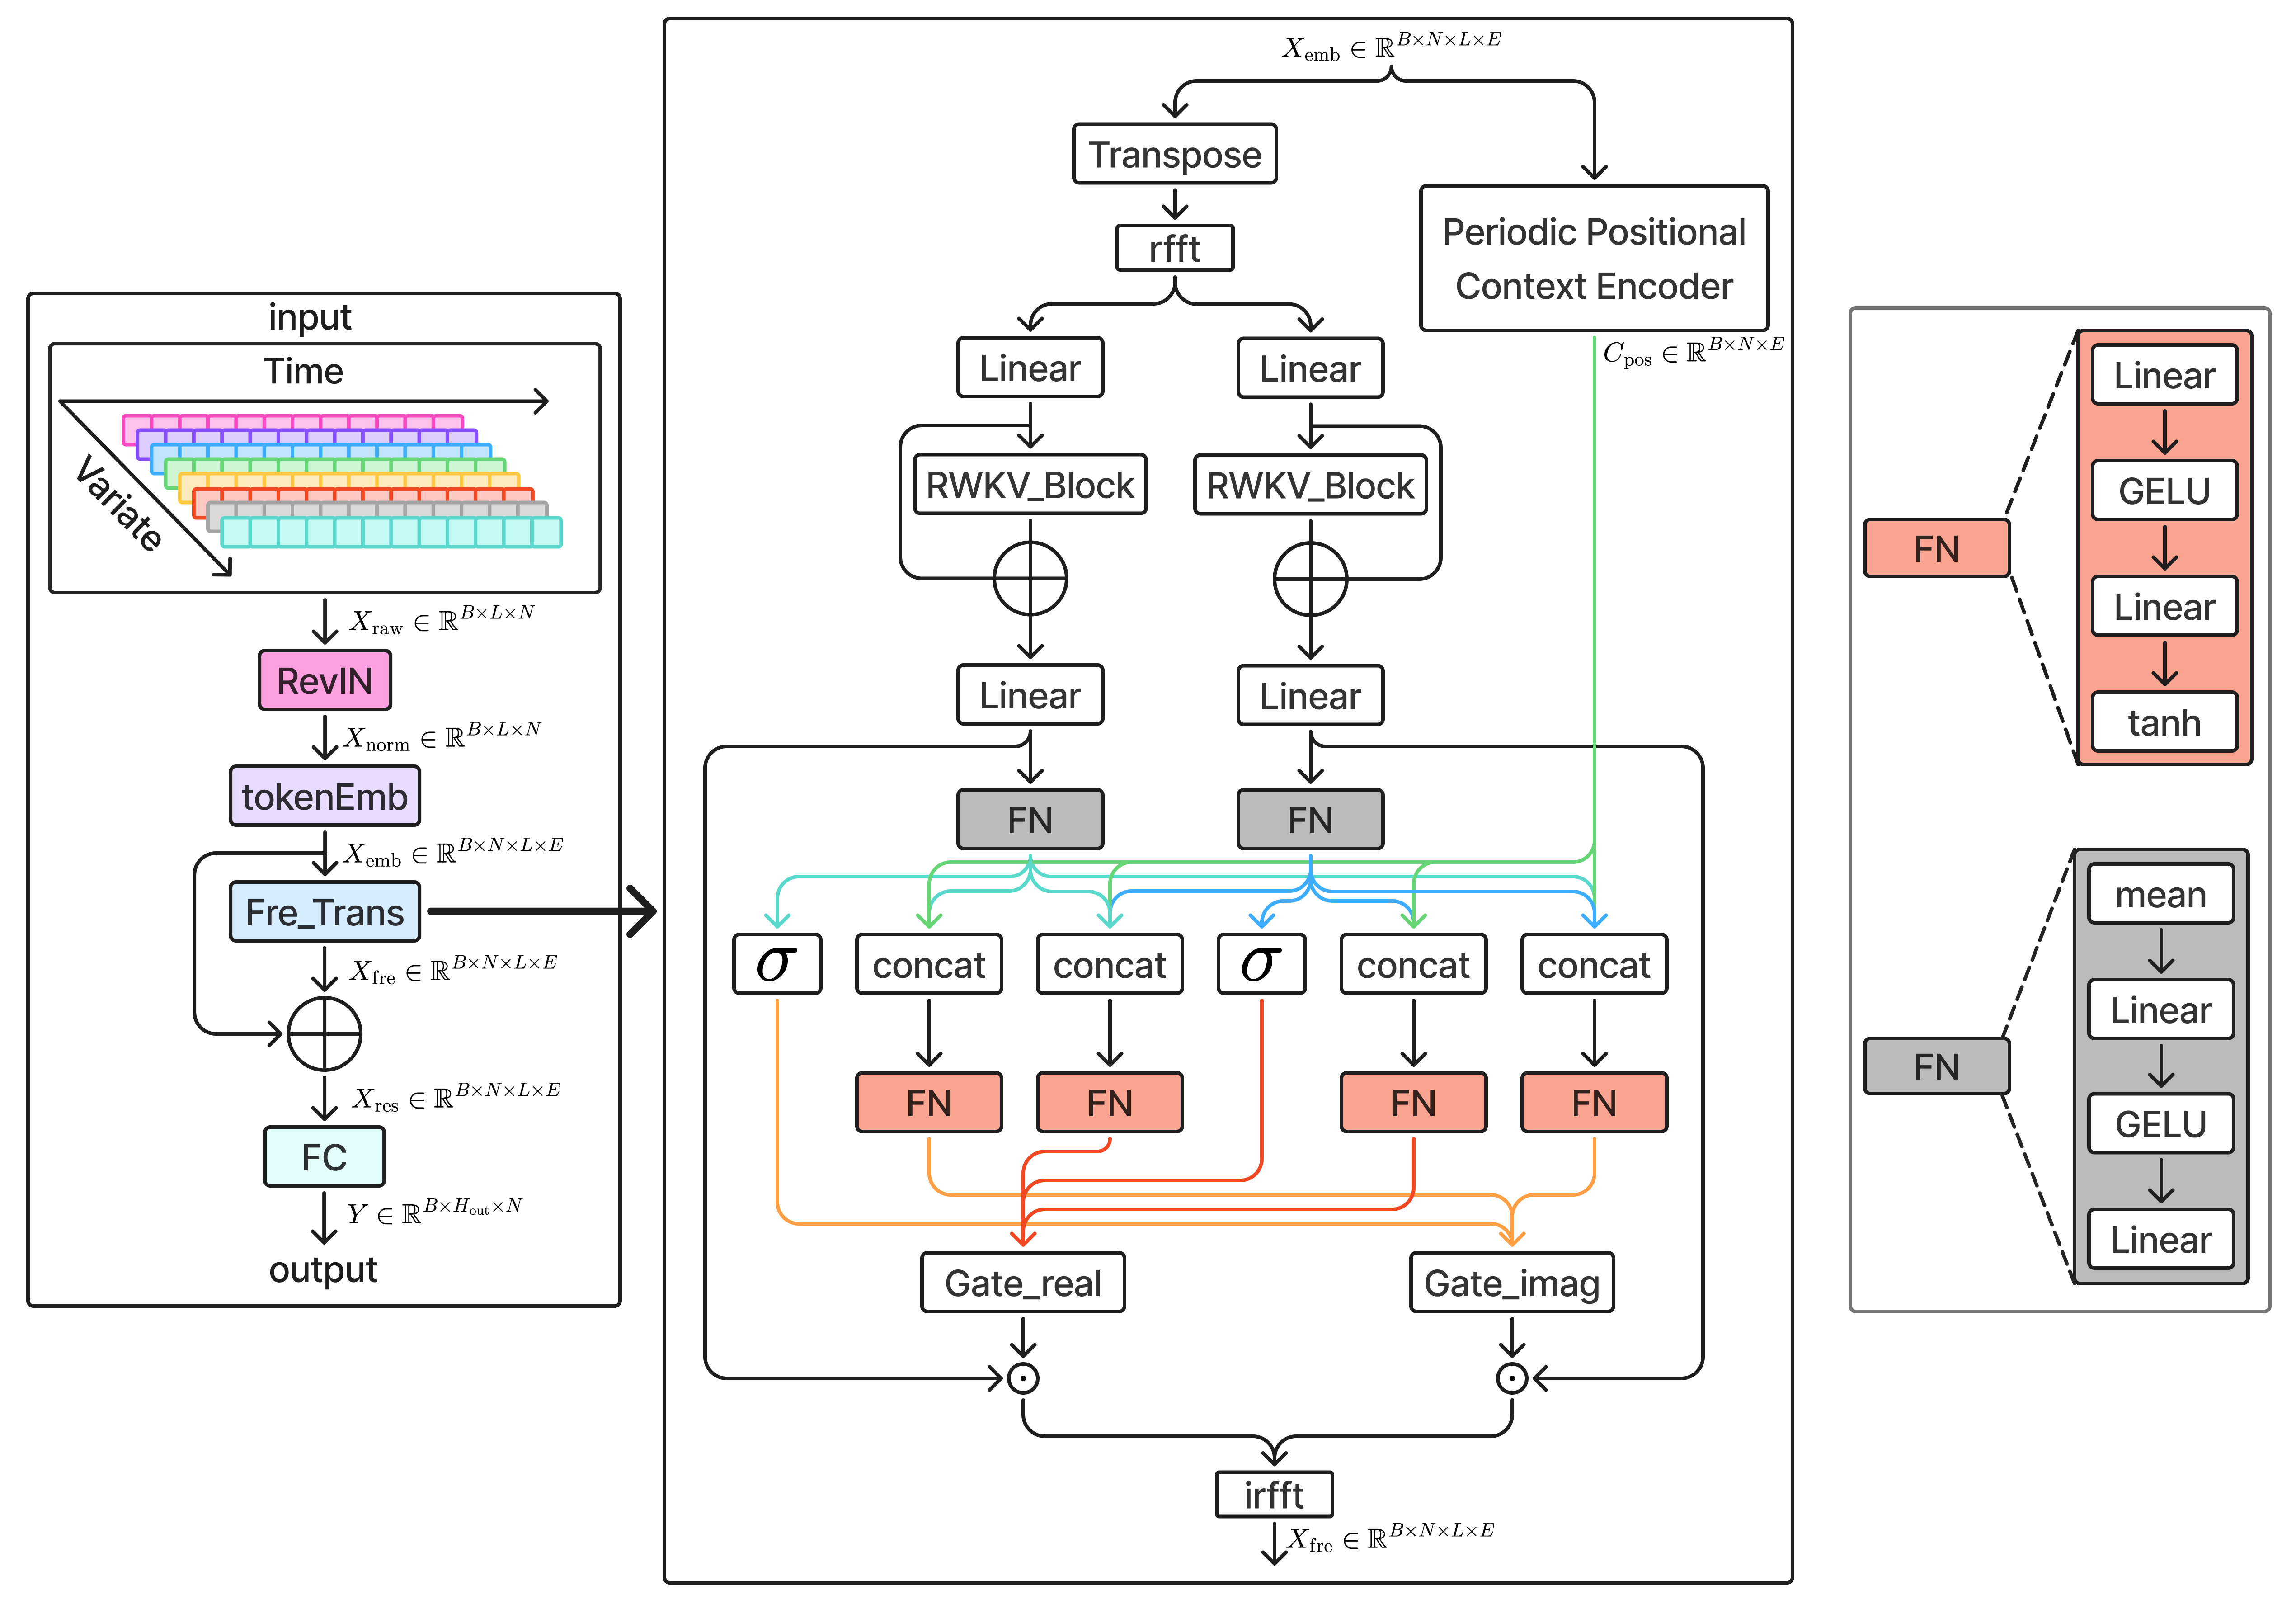
\includegraphics[width=\textwidth]{figs/fig_frwkvplus_main_simplified.png}
\caption{Simplified architecture of FRWKV+. The model applies RevIN and token embedding, sends the embedded sequence to the frequency transformation module, adds the transformed representation back to the embedding, and projects the result to the forecasting horizon. The frequency module contains real-imaginary RWKV encoding, cross-branch gating, PPCE-based periodic-position context extraction, signed gate correction, adaptive trust control, and inverse rFFT reconstruction.}
\label{fig:method_overview}
\end{figure}

\begin{figure}[p]
\centering
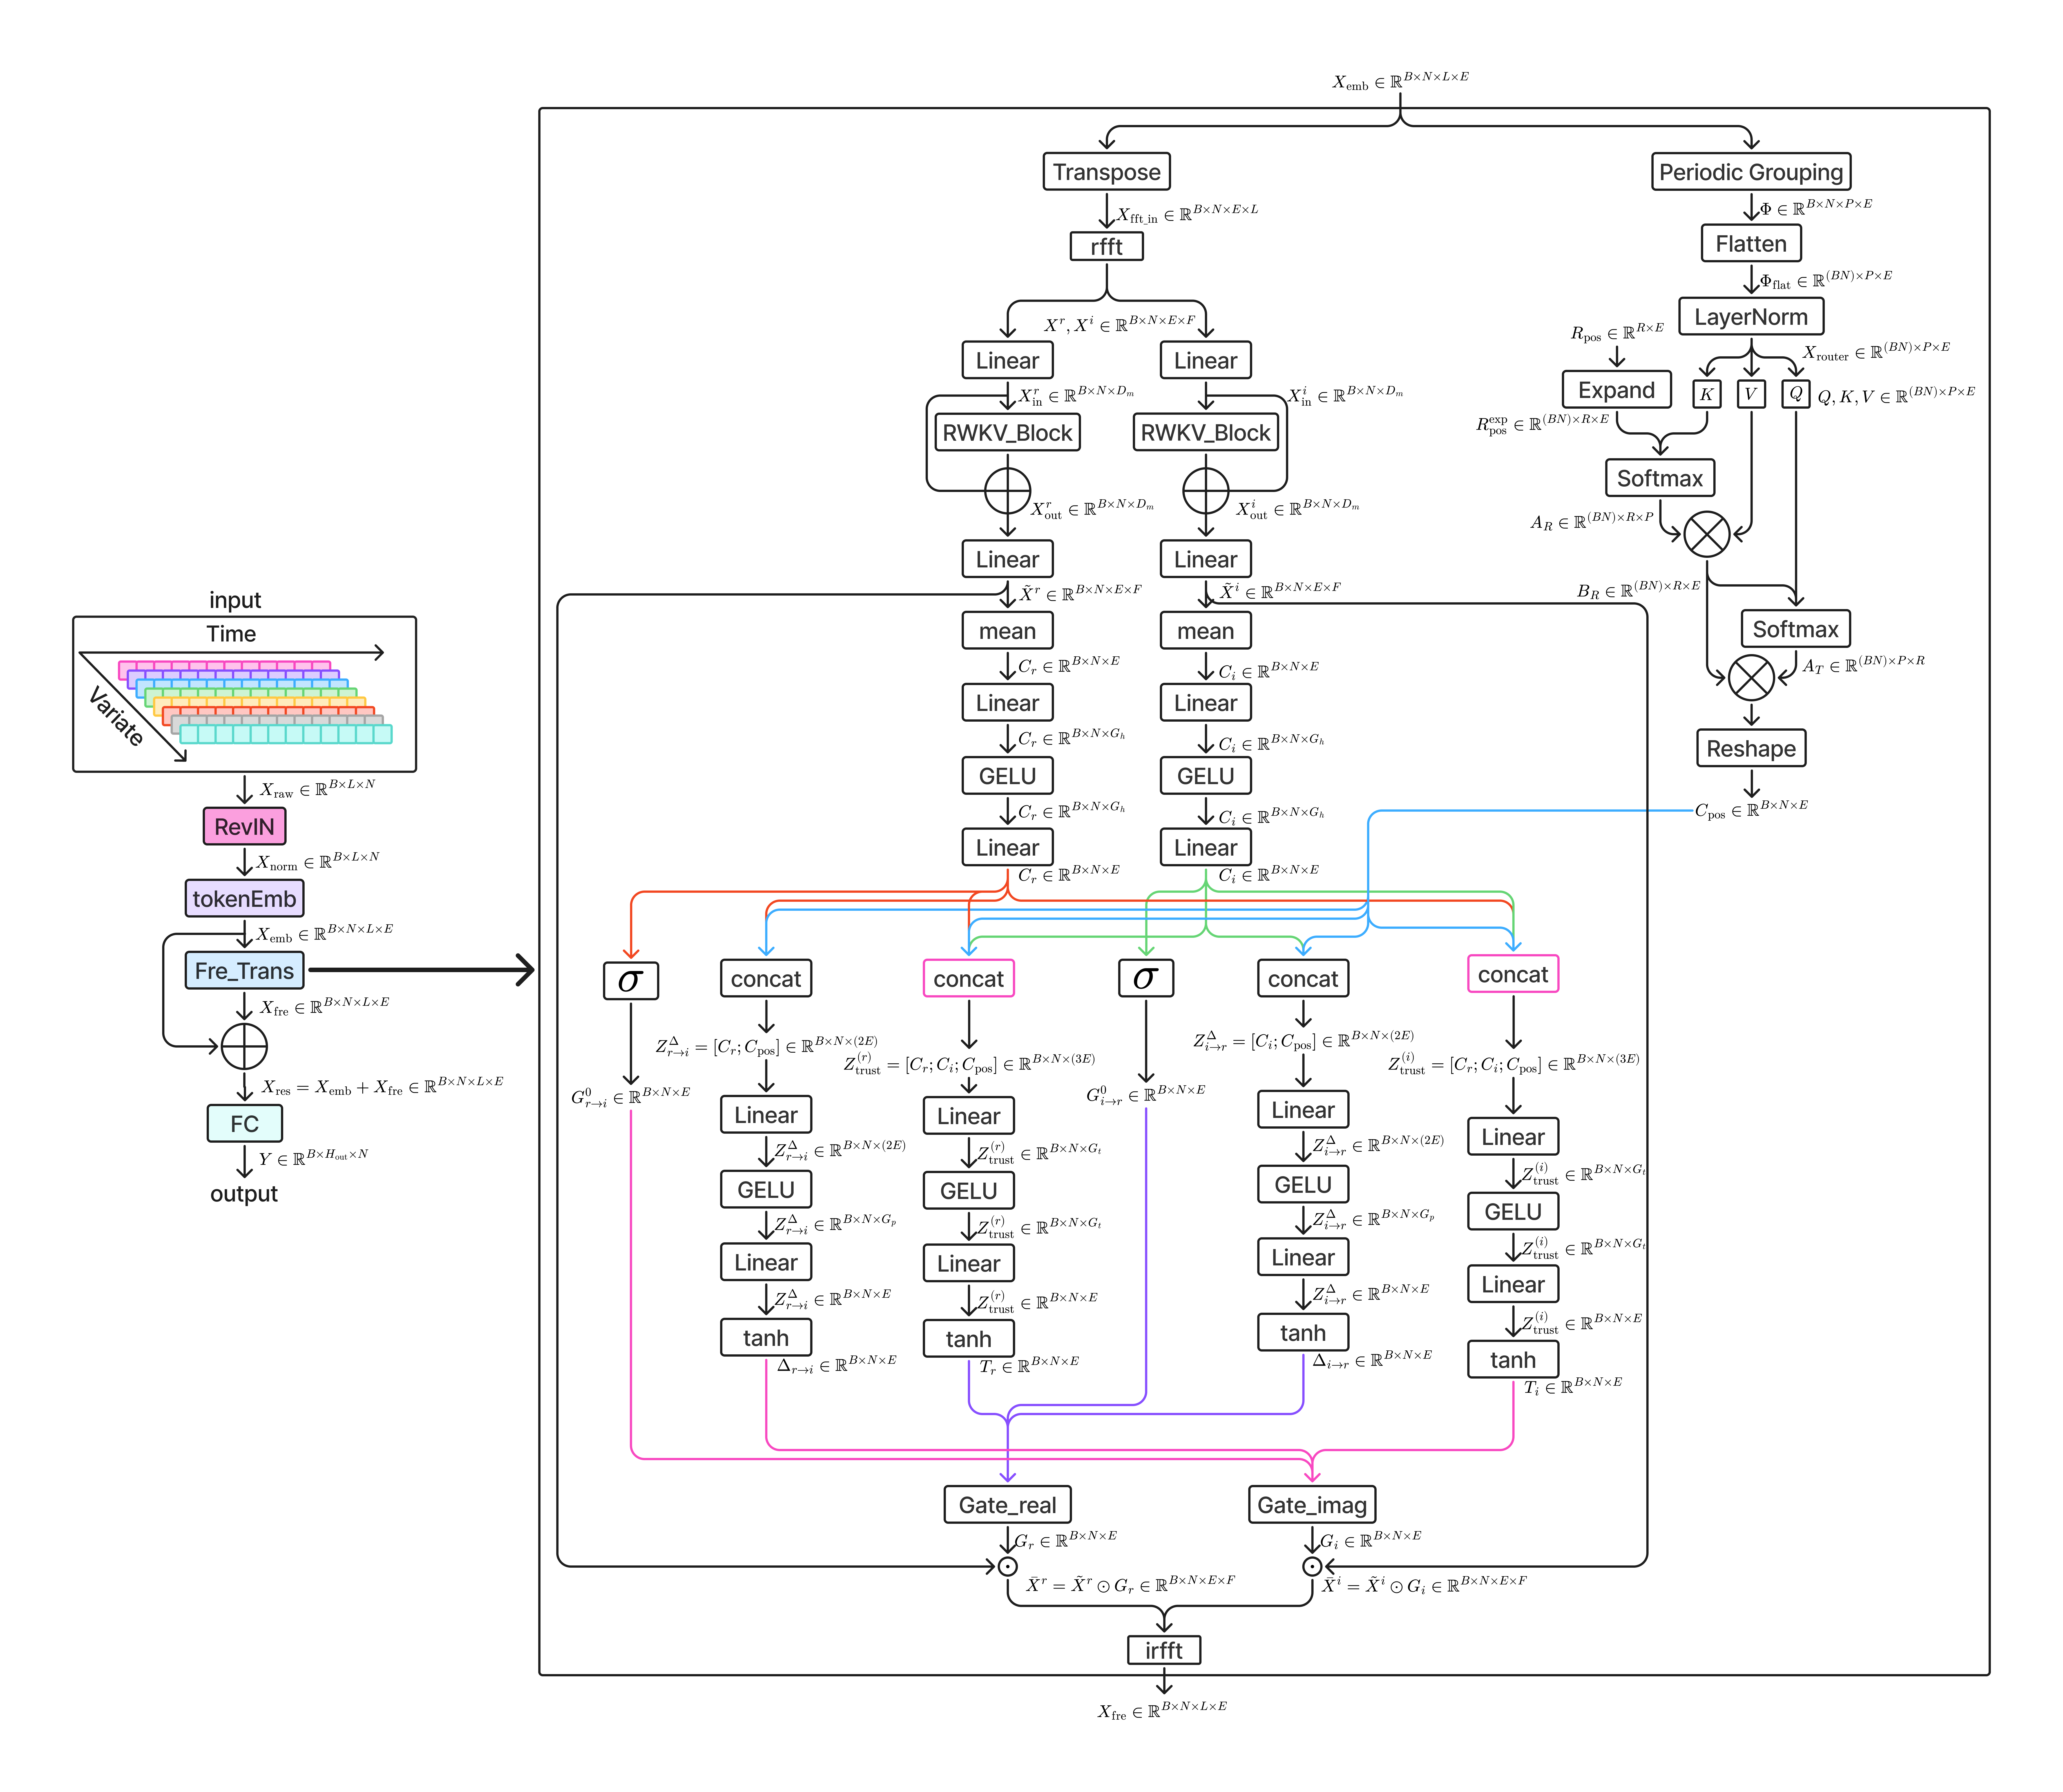
\includegraphics[width=\textwidth,height=0.84\textheight,keepaspectratio]{figs/fig_frwkvplus_main_full.png}
\caption{Tensor-level architecture of FRWKV+. The detailed diagram shows the rFFT path, the real and imaginary RWKV branches, the branch context vectors $C_r$ and $C_i$, the PPCE context $C_{\rm pos}$, the base gates $G^0_{r\to i}$ and $G^0_{i\to r}$, the signed corrections $\Delta_{r\to i}$ and $\Delta_{i\to r}$, the trust scores $T_r$ and $T_i$, and the final gates $G_r$ and $G_i$ that modulate the encoded real and imaginary responses before inverse rFFT.}
\label{fig:method_detail}
\end{figure}

\subsection{FRWKV backbone}
Let the input sequence be
\begin{equation}
X \in \mathbb{R}^{B \times T \times N},
\end{equation}
where $B$ is batch size, $T$ is input length, and $N$ is the number of variables. We first apply reversible instance normalization (RevIN) over the temporal axis to reduce scale variation across variables \cite{kim2022revin}:
\begin{equation}
\tilde{X}_{t,n} = \gamma_n \cdot \frac{X_{t,n} - \mu_n}{\sigma_n} + \beta_n.
\end{equation}

The normalized sequence is then lifted into a small embedding dimension before the frequency transform. For a learnable embedding vector $e \in \mathbb{R}^{D}$, we use
\begin{equation}
X_{\text{emb}}[b,n,t,d] = \tilde{X}[b,t,n] \cdot e_d,
\end{equation}
which gives $X_{\text{emb}} \in \mathbb{R}^{B \times N \times T \times D}$. Applying a real FFT along the temporal axis yields a complex frequency representation
\begin{equation}
Z = \operatorname{rFFT}(X_{\text{emb}}) = Z^{(r)} + i Z^{(i)},
\end{equation}
where $Z^{(r)}, Z^{(i)} \in \mathbb{R}^{B \times N \times D \times F}$ denote the real and imaginary frequency streams. The base FRWKV model \cite{yang2025frwkv} encodes these two streams with separate lightweight frequency branches. In simplified form, the linear state-update encoder inside each branch can be written as
\begin{equation}
S_\ell = A_\ell S_{\ell-1} + v_\ell (k_\ell^{\text{rep}})^\top,
\end{equation}
where $A_\ell$ is a decay-and-removal transition matrix and $v_\ell, k_\ell^{\text{rep}}$ are learned value and replacement-key representations. Figure~\ref{fig:rwkv_block} shows the RWKV block inherited from the original FRWKV backbone. The block uses shifted feature streams to generate receptance, key, value, gate, interpolation, and decay signals. The removal key and replacement key update a compact recurrent state, while the receptance stream reads from this state and the output gate controls the emitted response. This state-update form gives each frequency branch a linear-complexity sequence encoder. Each branch flattens the embedding-frequency axes, applies this RWKV encoder with residual connection, and reshapes the output back to the complex frequency layout. The processed real and imaginary responses are then recombined and mapped back to the time domain by inverse FFT.

\begin{figure}[p]
\centering
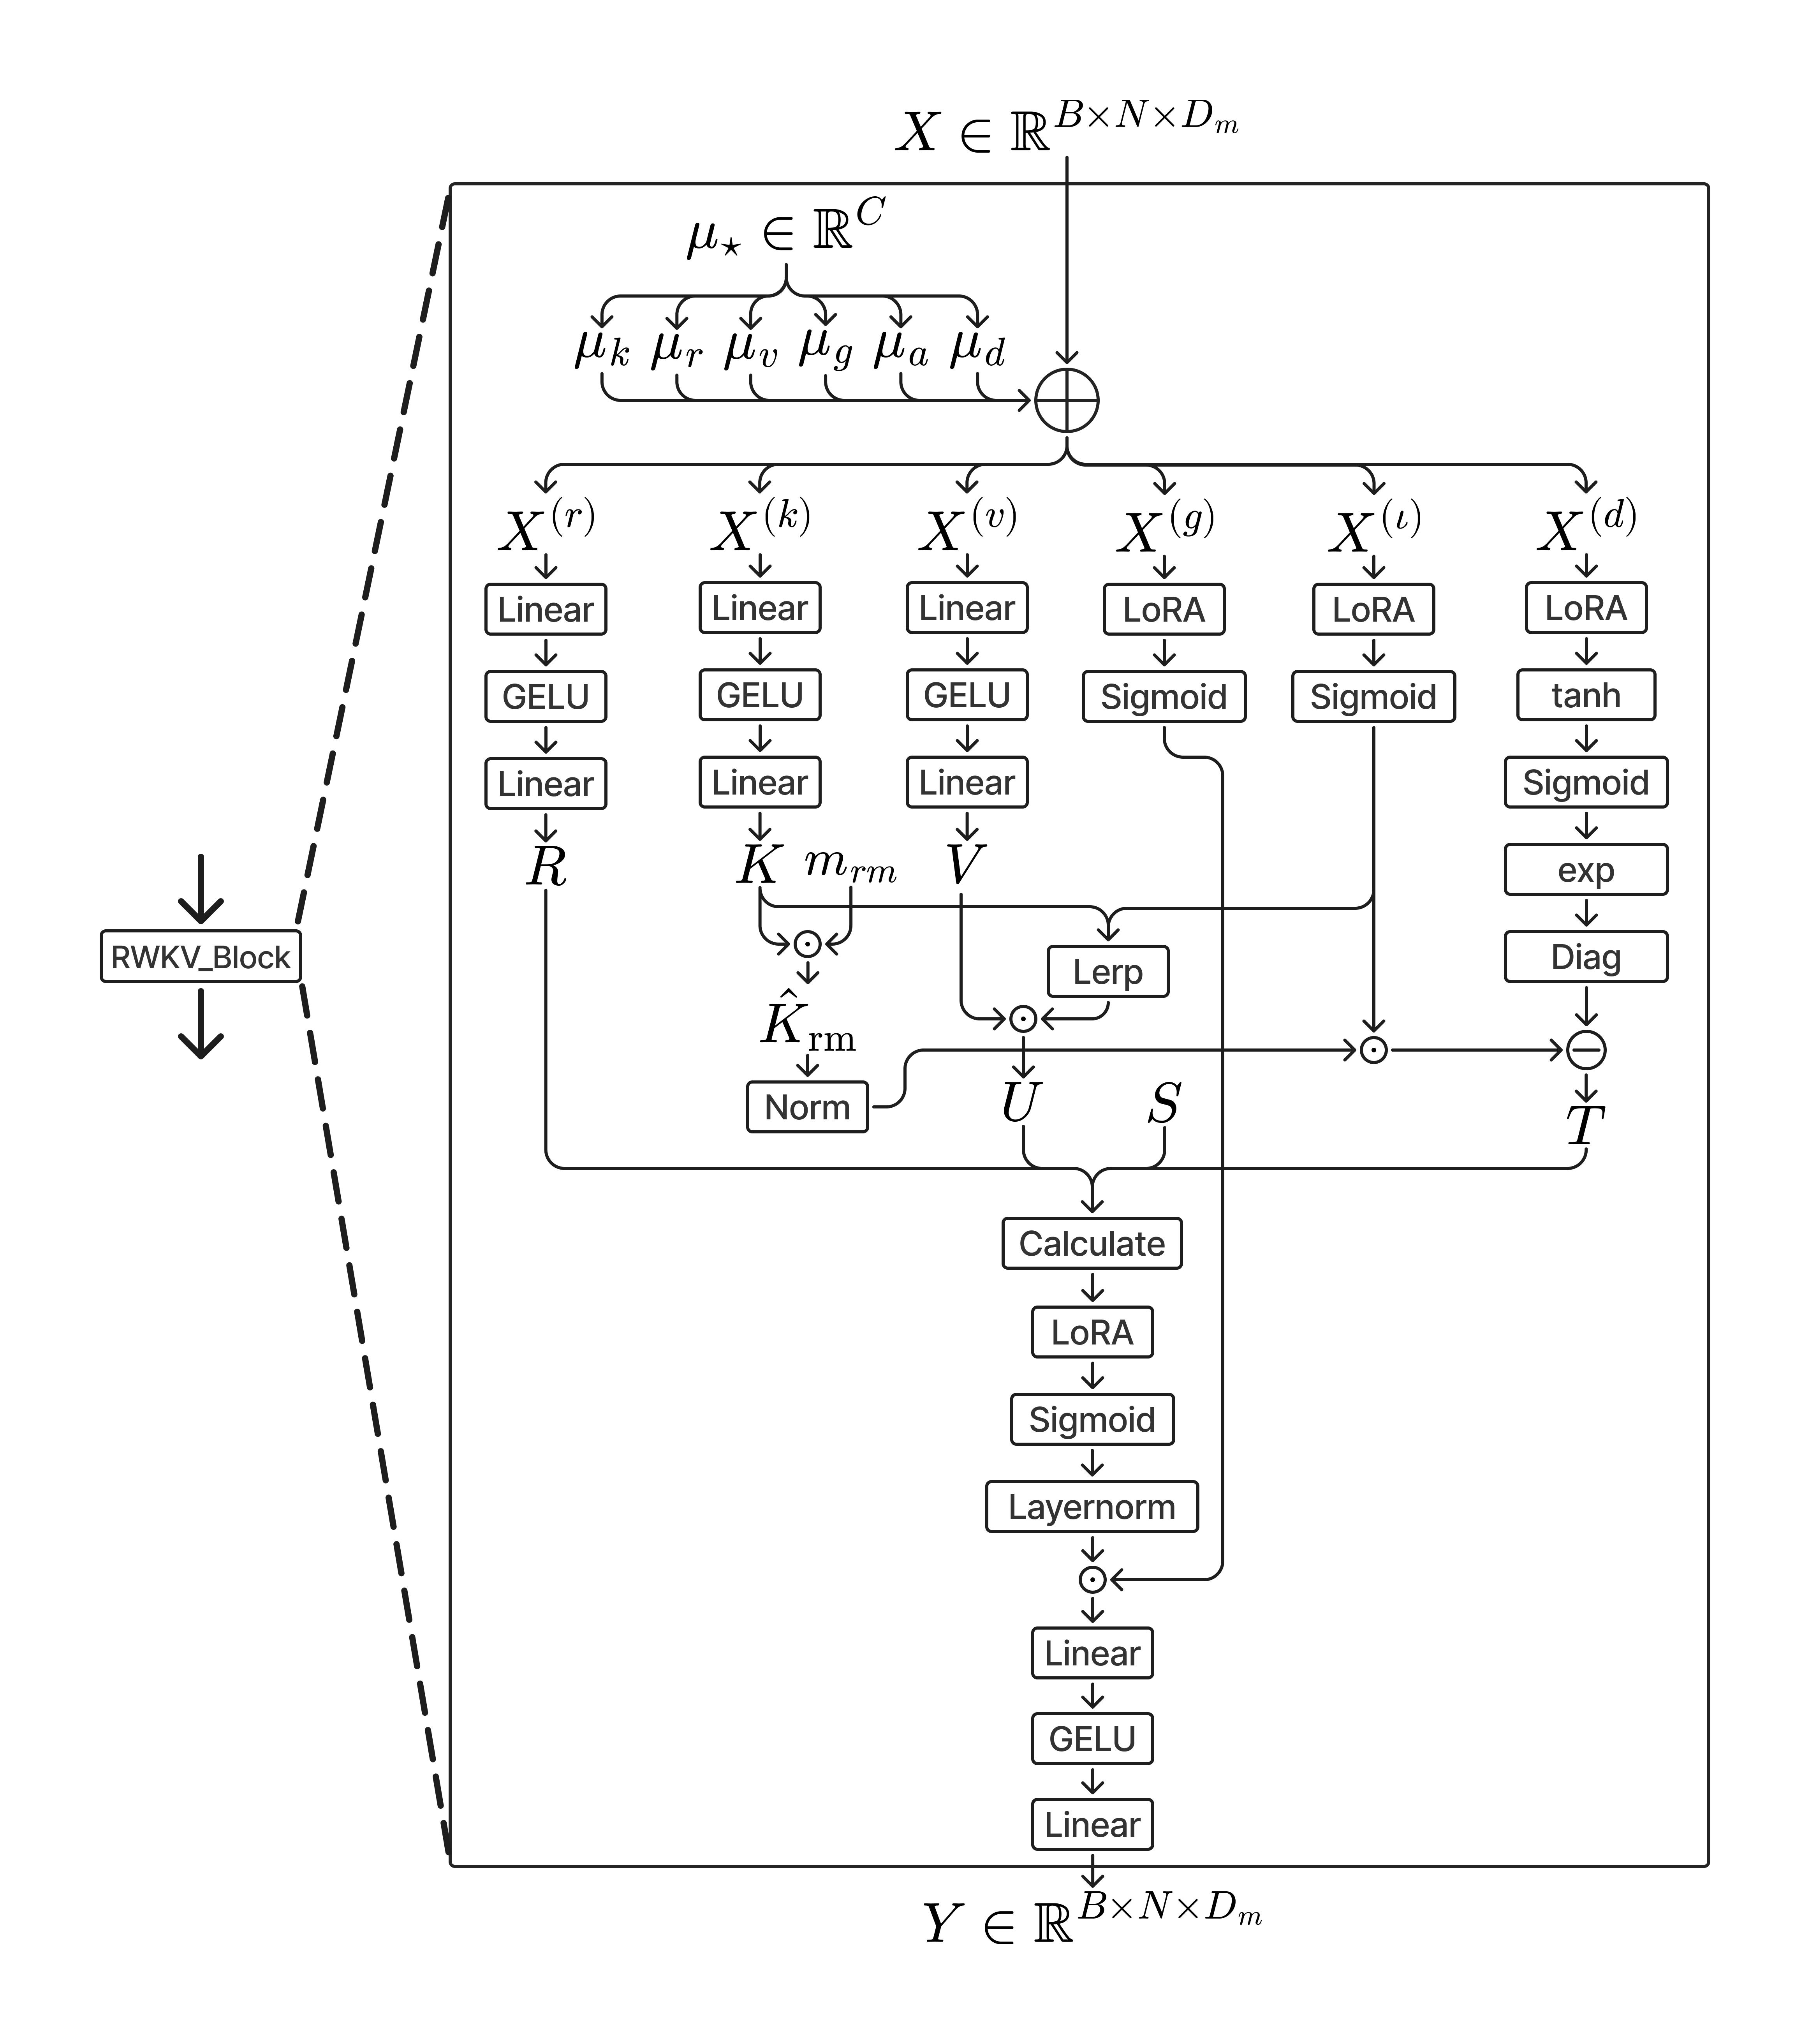
\includegraphics[width=0.82\textwidth,height=0.74\textheight,keepaspectratio]{figs/fig_rwkv_block.png}
\caption{RWKV block used by the FRWKV frequency branches. The block generates receptance, key, value, gate, interpolation, and decay streams from shifted features, updates a recurrent state with removal and replacement keys, and produces an output through normalization, gating, and projection. FRWKV+ keeps this efficient FRWKV block as the frequency-space backbone and adds selective branch interaction around it.}
\label{fig:rwkv_block}
\end{figure}

\subsection{CrossBranchGate}
The first enhancement addresses the interaction between the two complex frequency streams. Although $Z^{(r)}$ and $Z^{(i)}$ are processed by separate frequency branches for efficiency, they describe complementary parts of the same spectral representation. We therefore summarize the encoded responses along the frequency axis,
\begin{equation}
C_r = \operatorname{MeanFreq}(Y^{(r)}), \qquad C_i = \operatorname{MeanFreq}(Y^{(i)}),
\end{equation}
where $\operatorname{MeanFreq}$ averages over the frequency-bin axis. We then use the context from one branch to generate a gate for the other branch:
\begin{equation}
G_{i\to r}^0 = \sigma(\operatorname{MLP}_{i\to r}^{0}(C_i)), \qquad
G_{r\to i}^0 = \sigma(\operatorname{MLP}_{r\to i}^{0}(C_r)).
\end{equation}
Here the subscript denotes the source and target branches. The gate $G_{i\to r}^0$ is generated from the imaginary-branch context and modulates the real response, while $G_{r\to i}^0$ is generated from the real-branch context and modulates the imaginary response:
\begin{equation}
\bar{Y}^{(r)} = Y^{(r)} \odot (1 + G_{i\to r}^0), \qquad
\bar{Y}^{(i)} = Y^{(i)} \odot (1 + G_{r\to i}^0).
\end{equation}
This module gives the frequency branches a lightweight interaction path while preserving the separate-stream structure of the efficient backbone.

\subsection{Adaptive PhaseGate in FRWKV+}
The second enhancement makes the cross-branch gates aware of periodic position while keeping this information selective. We refer to the overall forecasting model as FRWKV+, and use Adaptive PhaseGate for the core mechanism that generates trust-controlled periodic-position corrections. In this implementation, the phase-related signal is represented as periodic-position context: it summarizes positions inside a chosen input period and uses this summary to correct the frequency-branch gates. This design reflects the empirical observation that periodic-position cues can be useful, but their reliability depends on the dataset and prediction horizon.

Figure~\ref{fig:ppce} shows the Periodic Positional Context Encoder. PPCE is the module that turns the time-domain embedding into the periodic-position context $C_{\rm pos}$. Its role is deliberately narrow: it extracts a compact context that describes recurring positions inside a period, and this context is later used by Adaptive PhaseGate as correction evidence. It does not replace the frequency representation or directly overwrite the real and imaginary responses.

\begin{figure}[t]
\centering
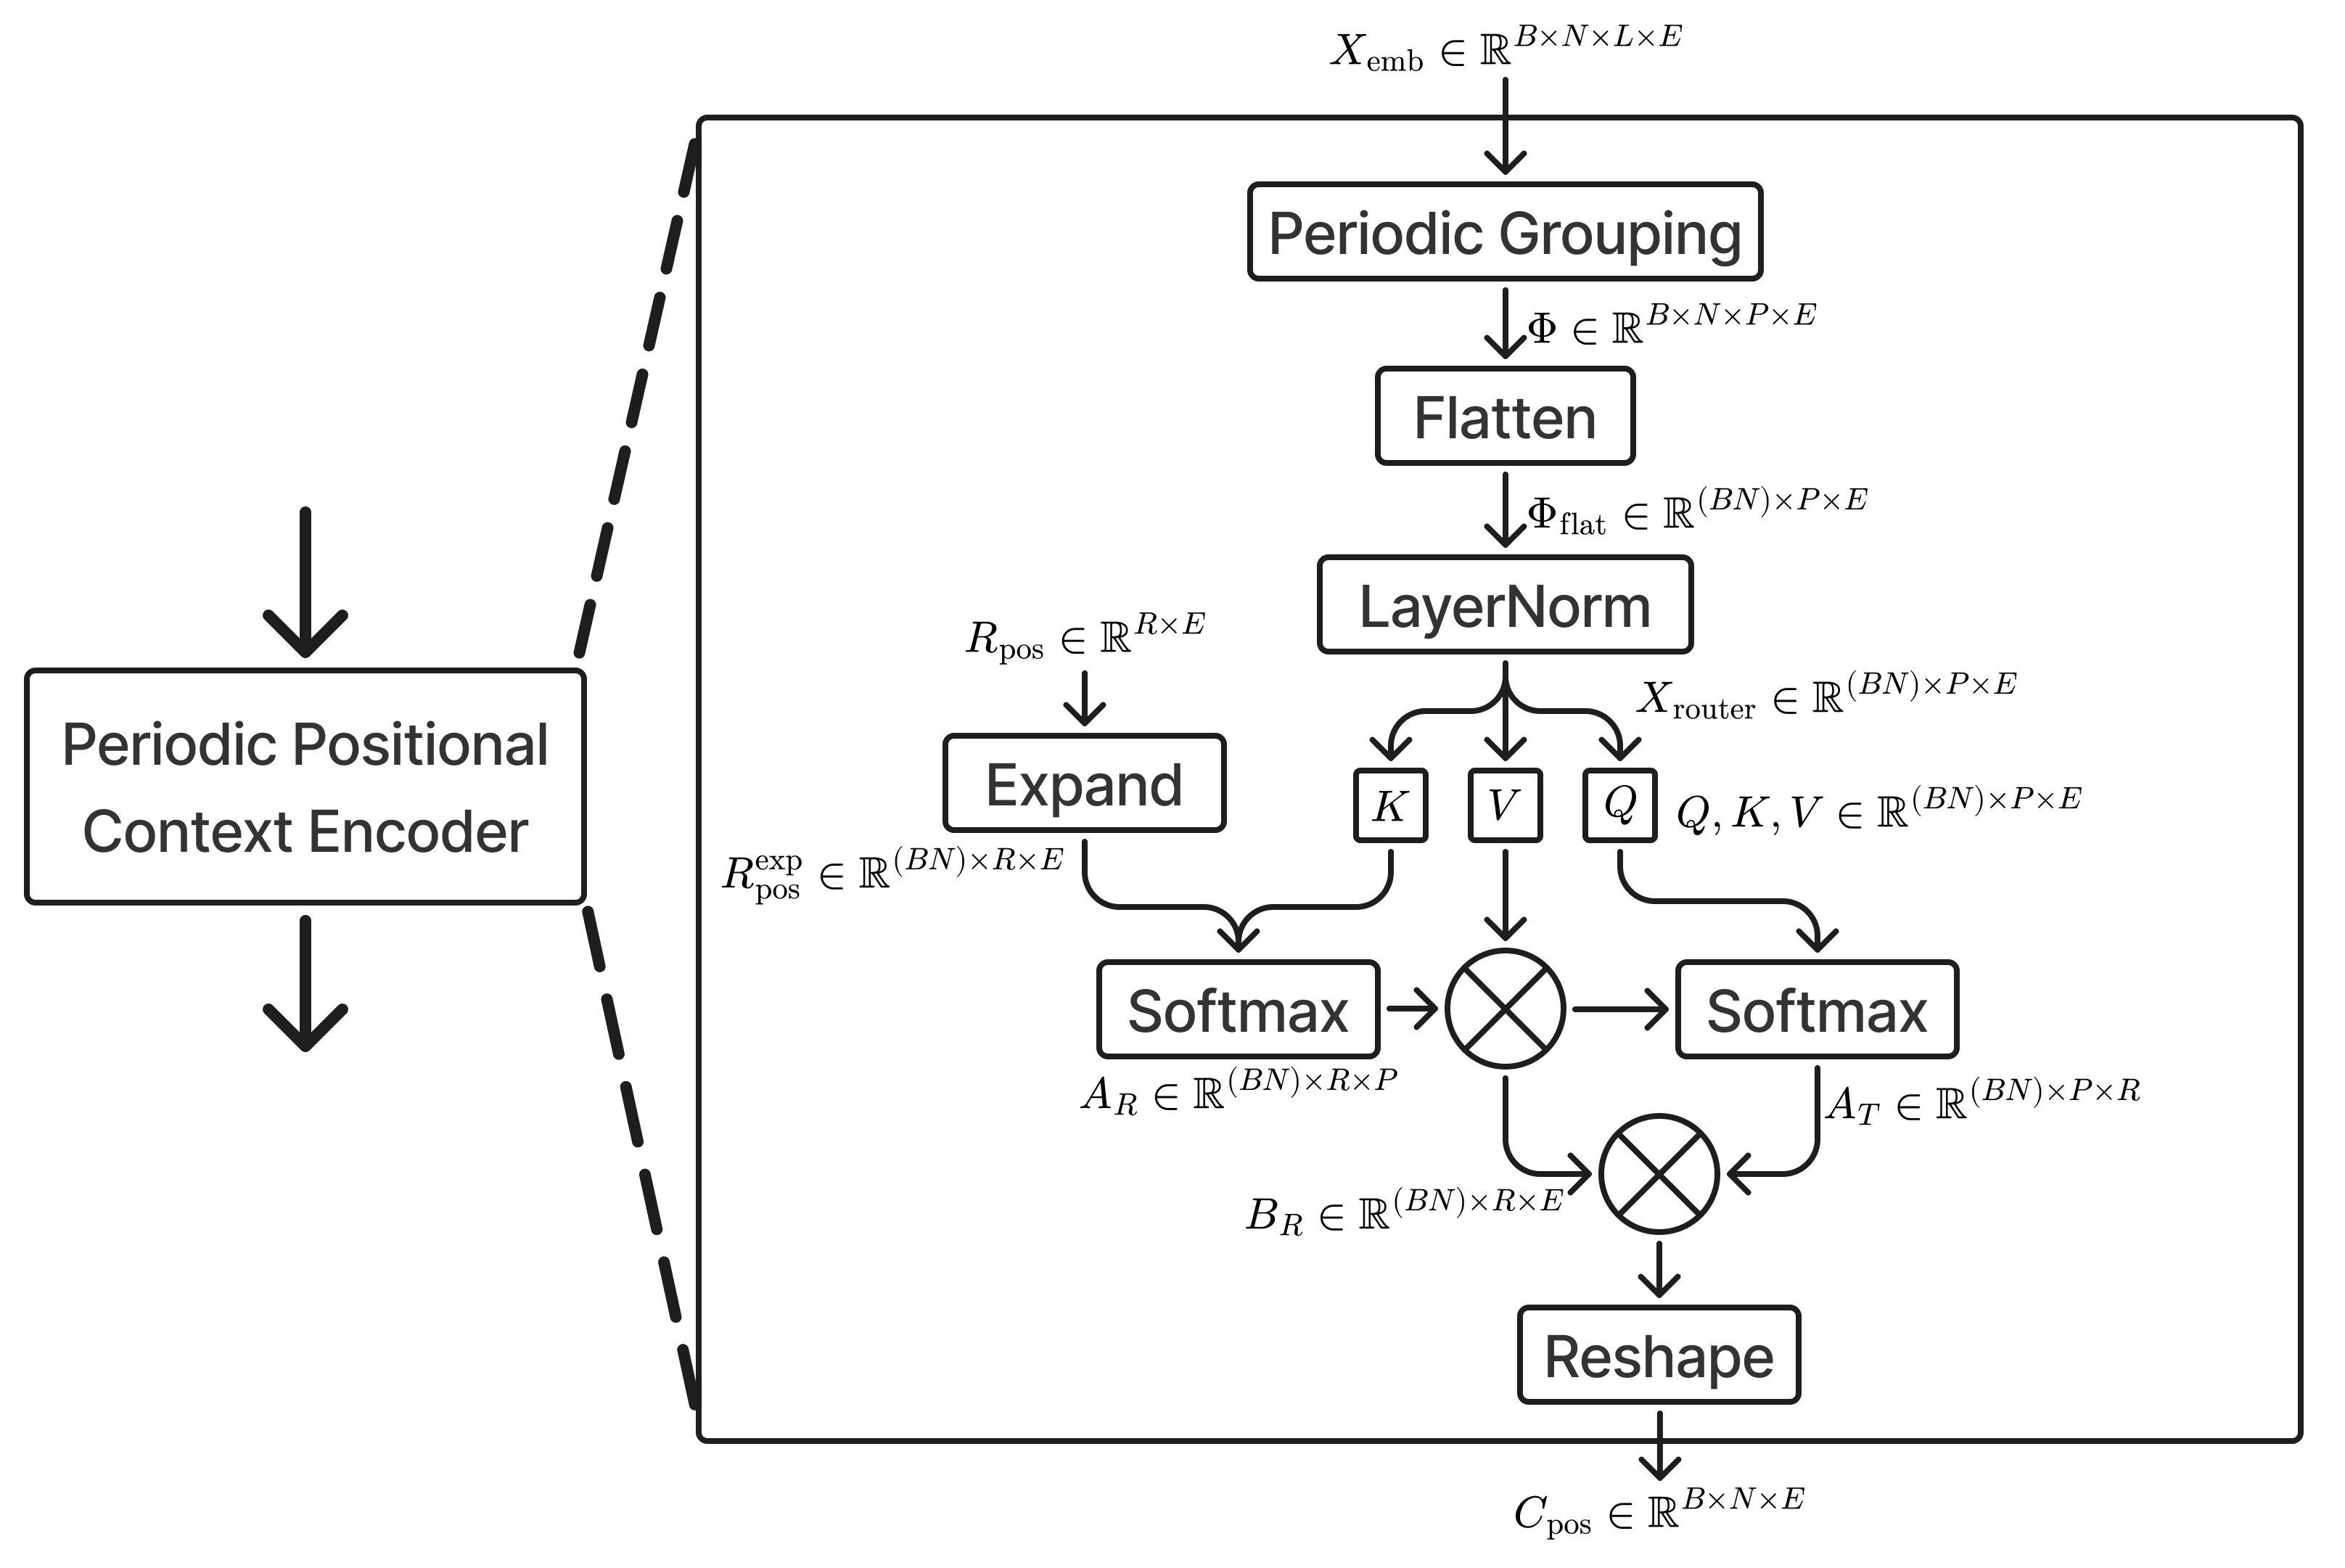
\includegraphics[width=\textwidth]{figs/fig_periodic_positional_context_encoder.png}
\caption{Periodic Positional Context Encoder. The embedded sequence is grouped by period position, flattened over sample and variable axes, normalized, and routed through learnable router tokens. The router aggregation produces $C_{\rm pos} \in \mathbb{R}^{B \times N \times D}$, a compact context vector for each sample and variable. This context provides periodic-position evidence for signed gate corrections and adaptive trust scores in FRWKV+.}
\label{fig:ppce}
\end{figure}

For a period-position length $P$, the embedded sequence $X_{\text{emb}}$ is circularly padded when necessary. Let $M=\lceil T/P\rceil$ denote the number of period groups after padding. The padded tensor is reshaped into $M$ repeated periods and averaged across repetitions:
\begin{equation}
\Phi[b,n,p,d] =
\frac{1}{M}\sum_{m=1}^{M} X_{\text{pad}}[b,n,m,p,d],
\qquad
\Phi \in \mathbb{R}^{B \times N \times P \times D}.
\end{equation}
This step produces one token for each position inside the chosen period. PPCE then flattens the sample and variable axes and applies layer normalization:
\begin{equation}
X_{\rm router} =
\operatorname{LN}(\operatorname{reshape}(\Phi))
\in \mathbb{R}^{(BN) \times P \times D}.
\end{equation}
With $R$ learnable router tokens $R_{\rm pos}\in\mathbb{R}^{R\times D}$, the router computes query, key, and value projections from the period-position tokens,
\begin{equation}
Q=X_{\rm router}W_Q,\qquad K=X_{\rm router}W_K,\qquad V=X_{\rm router}W_V,
\end{equation}
and first aggregates periodic-position evidence into router buffers:
\begin{equation}
A_R = \operatorname{softmax}\!\left(\frac{R_{\rm pos}^{\rm exp}K^\top}{\sqrt{D}}\right),
\qquad
B_R = A_R V.
\end{equation}
The token-to-router attention then returns the router evidence to the period-position tokens:
\begin{equation}
A_T = \operatorname{softmax}\!\left(\frac{Q B_R^\top}{\sqrt{D}}\right),
\qquad
U = A_T B_R.
\end{equation}
Finally, the routed periodic-position tokens are averaged over the period-position axis and projected to the context vector:
\begin{equation}
C_{\rm pos} = W_O\,\operatorname{MeanPos}(U),
\qquad
C_{\rm pos}\in\mathbb{R}^{B\times N\times D}.
\end{equation}
In the implementation this operator corresponds to \texttt{PeriodicPositionRouter}. The two-stage routing lets PPCE compress the $P$ period-position tokens through a small router set before returning a single context vector for each sample and variable.

The periodic-position context is used as an auxiliary correction source for the base cross-branch gates:
\begin{equation}
\Delta_{i\to r} = \tanh(\operatorname{MLP}_{i\to r}^{\Delta}([C_i, C_{\rm pos}])), \qquad
\Delta_{r\to i} = \tanh(\operatorname{MLP}_{r\to i}^{\Delta}([C_r, C_{\rm pos}])).
\end{equation}
The $\tanh$ output allows the correction to either increase or decrease the corresponding base gate, so periodic-position information acts as a directional adjustment rather than a one-way amplification.

Adaptive PhaseGate further learns how much of this correction should be admitted in FRWKV+. The branch-specific trust scores are
\begin{equation}
T_r = \sigma(\operatorname{MLP}^{(r)}_{\text{trust}}([C_r, C_i, C_{\rm pos}])),
\end{equation}
\begin{equation}
T_i = \sigma(\operatorname{MLP}^{(i)}_{\text{trust}}([C_r, C_i, C_{\rm pos}])).
\end{equation}
These scores are sample-, variable-, and embedding-channel-specific coefficients in $[0,1]$. They use the target-branch context, the source-branch context, and the periodic-position context as evidence for deciding whether the periodic correction is reliable for the current instance.

The final gates are
\begin{equation}
G_r = 1 + G_{i\to r}^0 + \alpha \, T_r \odot \Delta_{i\to r},
\end{equation}
\begin{equation}
G_i = 1 + G_{r\to i}^0 + \alpha \, T_i \odot \Delta_{r\to i}.
\end{equation}
The modulated frequency responses are then
\begin{equation}
\tilde{Y}^{(r)} = Y^{(r)} \odot G_r, \qquad
\tilde{Y}^{(i)} = Y^{(i)} \odot G_i.
\end{equation}
Here $\alpha$ is a learnable correction-strength parameter clipped to $[0,0.20]$ during the forward pass. The correction MLPs are initialized near zero, and the trust MLPs use a low initial bias. Thus FRWKV+ starts close to the CrossBranchGate baseline and learns to use periodic-position correction only when it provides useful evidence. This trust-controlled formulation is the key difference between Adaptive PhaseGate and an unconditional periodic-position injection.

\clearpage

\section{Experiments}
\subsection{Experimental setup}
We evaluate all methods on seven standard long-term forecasting benchmarks commonly used in LSTF studies \cite{zhou2021informer,wu2021autoformer,zhou2022fedformer}: ETTh1, ETTh2, ETTm1, ETTm2, Weather, Exchange, and ILI. For ETTh1, ETTh2, ETTm1, ETTm2, Weather, and Exchange, the input length is fixed to 96 and the prediction horizons are 96, 192, 336, and 720. For ILI, we follow the standard illness forecasting protocol with input length 36 and prediction horizons 24, 36, 48, and 60. We report MSE and MAE as the primary evaluation metrics.

\begin{table}[t]
\centering
\caption{Dataset and forecasting protocol summary.}
\label{tab:dataset_summary}
\scriptsize
\setlength{\tabcolsep}{4pt}
\begin{tabular}{lccccc}
\toprule
Dataset & Timesteps & Variables & Granularity & Input length & Horizons \\
\midrule
ETTh1 & 17420 & 7 & 1 hour & 96 & 96, 192, 336, 720 \\
ETTh2 & 17420 & 7 & 1 hour & 96 & 96, 192, 336, 720 \\
ETTm1 & 69680 & 7 & 15 min & 96 & 96, 192, 336, 720 \\
ETTm2 & 69680 & 7 & 15 min & 96 & 96, 192, 336, 720 \\
Weather & 52696 & 21 & 10 min & 96 & 96, 192, 336, 720 \\
Exchange & 7588 & 8 & 1 day & 96 & 96, 192, 336, 720 \\
ILI & 966 & 7 & 1 week & 36 & 24, 36, 48, 60 \\
\bottomrule
\end{tabular}
\par\smallskip
\begin{minipage}{\textwidth}
\footnotesize \emph{Note:} Timesteps and variable counts are computed from the local benchmark files used in our experiments. All settings use multivariate forecasting with MSE and MAE as evaluation metrics.
\end{minipage}
\end{table}

For external comparisons, we report manuscript-level selected results from our documented FRWKV-family experiment pool under the same dataset splits and forecasting horizons. This protocol compares the final tuned forecasting system with strong external baselines. The selected results mainly come from FRWKV+ recipes, and cases where a lighter internal embedding or a closely related FRWKV-family variant gives the selected main-table value are explicitly marked. Supplementary records provide the seed, model family, configuration type, and metric values for the selected cells. To keep this tuned-system comparison separate from mechanism-level evidence, we also conduct a strict matched-seed family ablation.

For the internal family study, we compare five variants: FRWKV, CrossBranchGate, CrossBranchPhaseGate, FullContextDelta, and FRWKV+ (Adaptive PhaseGate). All five variants are evaluated on the same 28 dataset-horizon settings with the same 16 random seeds, and the resulting record set is complete with no missing runs. This matched protocol is used for winner counts, average ranks, dataset-level averages, and paired analyses. It is the main evidence for interpreting whether periodic-position correction is useful, where it helps, and where simpler or fuller-context variants are preferable.

\paragraph{Implementation details.}
All FRWKV-family manuscript recipes are trained with AdamW and a cosine annealing learning-rate schedule. The learning rate is set to $1\times 10^{-4}$ and the weight decay is $1\times 10^{-3}$ in the current manuscript recipe set. The maximum number of training epochs is setting dependent, with values between 30 and 90 across the selected FRWKV+ recipes, and early stopping uses a setting-specific patience between 5 and 15 epochs. In the implementation, early stopping is activated only after at least half of the scheduled epochs have elapsed and no new best update has been observed for the configured patience. The batch size is 32 for ETTh1, ETTh2, ETTm1, ETTm2, Weather, and Exchange, and 16 for ILI.

For the selected FRWKV+ recipes, the main hidden dimension is 512, the feed-forward dimension is 512, the number of heads is 8, and the frequency embedding size is 16. The number of encoder layers is 2 for most datasets and 3 for Weather. The temporal patch length and stride are setting dependent, using patch lengths 12 or 16 and strides 6 or 8. Periodic-position hyperparameters are also tuned by setting: the period-position length ranges from 6 to 96, the number of routers ranges from 1 to 8, the initial correction-strength parameter ranges from 0.01 to 0.10, and the initial trust bias ranges from -4.0 to -2.0. We therefore report these settings as recipe-level hyperparameters rather than as a single global configuration.

Training uses the implemented \texttt{WeightedSequenceLoss} with \texttt{loss\_mode=L1} and \texttt{lossfun\_alpha=0.5} for the current manuscript FRWKV+ recipes. This objective is a weighted L1, or weighted MAE-style, sequence loss: for a prediction horizon index $t$, the per-step absolute error is multiplied by the horizon weight $(t+1)^{-0.5}$ before averaging over the sequence and variables. Thus the training criterion is aligned with MAE-style robustness while giving larger weight to earlier forecast steps. MSE and MAE are both reported for evaluation, but the optimized objective in the manuscript recipes is this weighted L1 sequence loss.

\subsection{Main comparison against strong baselines}
Tables~\ref{tab:keypointsa} and~\ref{tab:keypointsb} compare our FRWKV-family forecasting system with strong external baselines across the seven benchmarks. The ``FRWKV+ (Ours)'' column reports the selected manuscript result from a curated FRWKV-family experiment pool under the same forecasting protocol. Most entries are produced by the default FRWKV+ recipes, whose core mechanism is Adaptive PhaseGate. When a selected entry comes from a closely related FRWKV-family configuration rather than the default FRWKV+ recipe, the table note marks that selection explicitly. This convention keeps the external comparison faithful to the reported numbers while avoiding the stronger claim that every main-table cell is produced by a single fixed architecture.

The purpose of the main comparison is to show that the proposed frequency-space family is competitive with representative linear-attention-style, large-model-based, lightweight linear, and Former-family forecasters. RWKV-TS and S-D-Mamba represent efficient recurrent or state-space sequence models \cite{hou2024rwkvts,wang2025smamba}; T3Time, TimeCMA, TimeLLM, and Chronos-2 represent large-model-based forecasting baselines \cite{chowdhury2025t3time,liu2025timecma,jin2024timellm,ansari2025chronos2}; DLinear provides a lightweight linear reference \cite{zeng2023dlinear}; and UniTime, iTransformer, PatchTST, FreTS, and MP-Former cover the Former-family comparison group \cite{liu2024unitime,liu2024itransformer,nie2023patchtst,yi2023frets,naghashi2025multipatchformer}. Local reproductions are explicitly indicated in the table notes; other external baseline values follow the cited papers, official repositories, or compatible evaluation records collected for the KBS comparison.

The external comparison is therefore a tuned-system comparison. Mechanism-level conclusions about cross-branch interaction, periodic-position correction, adaptive trust, and dataset-dependent regimes are based on the matched 16-seed ablation in Table~\ref{tab:ablation}.

\begin{table}[t]
\centering
\caption{Main comparison across seven benchmarks with linear-attention-style and LLM-based baselines (A).}
\label{tab:keypointsa}
\small
\setlength{\tabcolsep}{2.85pt}
\renewcommand{\arraystretch}{0.96}
\resizebox{\textwidth}{!}{%
\begin{tabular}{c|c|cc|cc|cc|cc|cc|cc|cc}
\toprule
\multirow{2}{*}{\textbf{Dataset}} & \multirow{2}{*}{\textbf{Horizon}} & \multicolumn{2}{c|}{\shortstack{\textbf{FRWKV+}\\\textbf{(Ours)}}} & \multicolumn{2}{c|}{\shortstack{\textbf{RWKV-TS}\textsuperscript{LA}\\\textbf{(2024)}}} & \multicolumn{2}{c|}{\shortstack{\textbf{S-D-Mamba}\textsuperscript{LA}\\\textbf{(2024)}}} & \multicolumn{2}{c|}{\shortstack{\textbf{T3Time}\textsuperscript{LM}\\\textbf{(2025)}}} & \multicolumn{2}{c|}{\shortstack{\textbf{TimeCMA}\textsuperscript{LM}\\\textbf{(2025)}}} & \multicolumn{2}{c|}{\shortstack{\textbf{TimeLLM}\textsuperscript{LM}\\\textbf{(2024)}}} & \multicolumn{2}{c}{\shortstack{\textbf{Chronos-2}\textsuperscript{LM}\\\textbf{(2025)}}} \\
& & MSE & MAE & MSE & MAE & MSE & MAE & MSE & MAE & MSE & MAE & MSE & MAE & MSE & MAE \\
\midrule
\multirow{5}{*}{ETTm1}
& 96 & \textbf{\textcolor{red}{0.308}} & \textbf{\textcolor{red}{0.339}} & 0.327 & 0.365 & 0.331 & 0.368 & \textbf{\textcolor{red}{0.308}} & 0.354 & \textbf{0.312} & \textbf{0.351} & 0.359 & 0.381 & 0.593 & 0.452 \\
& 192 & \textbf{\textcolor{red}{0.357}} & \textbf{\textcolor{red}{0.370}} & 0.369 & 0.388 & 0.378 & 0.393 & \textbf{\textcolor{red}{0.357}} & 0.381 & \textbf{0.361} & \textbf{0.378} & 0.383 & 0.393 & 0.609 & 0.467 \\
& 336 & \textbf{0.389} & \textbf{\textcolor{red}{0.391}} & 0.402 & 0.409 & 0.410 & 0.414 & \textbf{\textcolor{red}{0.382}} & \textbf{0.400} & 0.392 & 0.401 & 0.416 & 0.414 & 0.619 & 0.482 \\
& 720 & \textbf{0.452} & \textbf{\textcolor{red}{0.427}} & 0.461 & 0.446 & 0.474 & 0.451 & \textbf{\textcolor{red}{0.442}} & \textbf{0.437} & 0.453 & 0.438 & 0.483 & 0.449 & 0.648 & 0.508 \\
& Avg & \textbf{0.377} & \textbf{\textcolor{red}{0.382}} & 0.390 & 0.402 & 0.398 & 0.407 & \textbf{\textcolor{red}{0.372}} & 0.393 & 0.380 & \textbf{0.392} & 0.410 & 0.409 & 0.617 & 0.478 \\
\midrule
\multirow{5}{*}{ETTm2}
& 96 & \textbf{\textcolor{red}{0.171}} & \textbf{\textcolor{red}{0.249}} & 0.178 & 0.270 & 0.182 & 0.266 & \textbf{0.172} & \textbf{0.254} & 0.173 & 0.258 & 0.193 & 0.280 & 0.210 & 0.273 \\
& 192 & \textbf{\textcolor{red}{0.233}} & \textbf{\textcolor{red}{0.291}} & 0.251 & 0.314 & 0.252 & 0.313 & \textbf{0.237} & \textbf{0.300} & 0.238 & 0.301 & 0.257 & 0.318 & 0.274 & 0.314 \\
& 336 & \textbf{\textcolor{red}{0.292}} & \textbf{\textcolor{red}{0.328}} & 0.310 & 0.353 & 0.313 & 0.349 & 0.306 & \textbf{0.337} & \textbf{0.297} & 0.338 & 0.317 & 0.353 & 0.340 & 0.355 \\
& 720 & \textbf{\textcolor{red}{0.390}} & \textbf{\textcolor{red}{0.388}} & 0.407 & 0.414 & 0.413 & 0.405 & 0.400 & 0.398 & \textbf{0.393} & \textbf{0.394} & 0.419 & 0.411 & 0.448 & 0.412 \\
& Avg & \textbf{\textcolor{red}{0.272}} & \textbf{\textcolor{red}{0.314}} & 0.287 & 0.338 & 0.290 & 0.333 & 0.279 & \textbf{0.322} & \textbf{0.275} & 0.323 & 0.296 & 0.340 & 0.318 & 0.339 \\
\midrule
\multirow{5}{*}{ETTh1}
& 96 & \textbf{\textcolor{red}{0.371}} & \textbf{\textcolor{red}{0.388}} & 0.384 & 0.400 & 0.388 & 0.406 & \textbf{\textcolor{red}{0.371}} & 0.397 & \textbf{0.373} & \textbf{0.391} & 0.398 & 0.410 & 0.424 & 0.397 \\
& 192 & \textbf{0.424} & \textbf{\textcolor{red}{0.419}} & 0.445 & 0.433 & 0.445 & 0.441 & \textbf{\textcolor{red}{0.411}} & \textbf{0.421} & 0.427 & \textbf{0.421} & 0.451 & 0.440 & 0.484 & 0.431 \\
& 336 & 0.462 & \textbf{\textcolor{red}{0.441}} & 0.488 & 0.459 & 0.490 & 0.465 & \textbf{\textcolor{red}{0.448}} & \textbf{\textcolor{red}{0.441}} & \textbf{0.458} & \textbf{0.448} & 0.473 & 0.451 & 0.536 & 0.456 \\
& 720 & 0.463$^\ddagger$ & \textbf{\textcolor{red}{0.460}} & 0.496 & 0.484 & 0.506 & 0.497 & \textbf{\textcolor{red}{0.441}} & \textbf{\textcolor{red}{0.460}} & \textbf{0.449} & \textbf{\textcolor{red}{0.460}} & 0.469 & \textbf{0.470} & 0.526 & 0.471 \\
& Avg & 0.430 & \textbf{\textcolor{red}{0.427}} & 0.453 & 0.444 & 0.457 & 0.452 & \textbf{\textcolor{red}{0.418}} & \textbf{0.430} & \textbf{0.423} & 0.431 & 0.448 & 0.443 & 0.492 & 0.439 \\
\midrule
\multirow{5}{*}{ETTh2}
& 96 & \textbf{\textcolor{red}{0.278}} & \textbf{\textcolor{red}{0.327}} & 0.311 & 0.364 & 0.297 & 0.349 & \textbf{\textcolor{red}{0.278}} & 0.338 & \textbf{0.286} & \textbf{0.336} & 0.295 & 0.345 & 0.317 & 0.345 \\
& 192 & \textbf{0.358} & \textbf{\textcolor{red}{0.379}} & 0.376 & 0.410 & 0.378 & 0.399 & \textbf{\textcolor{red}{0.351}} & 0.389 & 0.363 & \textbf{0.387} & 0.386 & 0.399 & 0.413 & 0.400 \\
& 336 & 0.396 & \textbf{0.410} & \textbf{0.390} & 0.420 & 0.425 & 0.435 & \textbf{\textcolor{red}{0.358}} & \textbf{\textcolor{red}{0.398}} & 0.406 & 0.421 & 0.419 & 0.429 & 0.449 & 0.434 \\
& 720 & \textbf{0.409} & \textbf{\textcolor{red}{0.430}} & 0.421 & 0.454 & 0.432 & 0.448 & \textbf{\textcolor{red}{0.404}} & \textbf{0.433} & 0.417 & 0.438 & 0.425 & 0.442 & 0.443 & 0.442 \\
& Avg & \textbf{0.360} & \textbf{\textcolor{red}{0.387}} & 0.375 & 0.412 & 0.383 & 0.408 & \textbf{\textcolor{red}{0.348}} & \textbf{0.390} & 0.372 & 0.397 & 0.381 & 0.404 & 0.406 & 0.405 \\
\midrule
\multirow{5}{*}{Weather}
& 96 & \textbf{\textcolor{red}{0.156}} & \textbf{\textcolor{red}{0.194}} & 0.178 & 0.221 & 0.165 & \textbf{0.209} & \textbf{0.162} & 0.210 & 0.167 & 0.211 & 0.198 & 0.235 & 0.244 & 0.230 \\
& 192 & \textbf{\textcolor{red}{0.205}} & \textbf{\textcolor{red}{0.238}} & 0.219 & 0.256 & 0.215 & 0.255 & \textbf{0.211} & \textbf{0.253} & 0.212 & \textbf{0.253} & 0.240 & 0.269 & 0.273 & 0.270 \\
& 336 & \textbf{\textcolor{red}{0.264}} & \textbf{\textcolor{red}{0.282}} & 0.275 & 0.297 & 0.273 & 0.296 & \textbf{0.267} & 0.293 & 0.270 & \textbf{0.292} & 0.295 & 0.308 & 0.319 & 0.306 \\
& 720 & \textbf{0.342$^\S$} & \textbf{\textcolor{red}{0.335}} & 0.353 & 0.347 & 0.353 & 0.349 & \textbf{\textcolor{red}{0.335}} & \textbf{0.346} & 0.350 & 0.348 & 0.368 & 0.353 & 0.393 & 0.357 \\
& Avg & \textbf{\textcolor{red}{0.242}} & \textbf{\textcolor{red}{0.262}} & 0.256 & 0.280 & 0.252 & 0.277 & \textbf{0.244} & \textbf{0.275} & 0.250 & 0.276 & 0.275 & 0.291 & 0.307 & 0.291 \\
\midrule
\multirow{5}{*}{ILI}
& 24 & \textbf{\textcolor{red}{1.432}} & \textbf{\textcolor{red}{0.721}} & 2.036 & 0.916 & 2.675 & 1.074 & \textbf{1.583} & \textbf{0.802} & 1.996 & 0.998 & 2.383 & 1.004 & 7.511 & 1.651 \\
& 36 & \textbf{\textcolor{red}{1.392}} & \textbf{\textcolor{red}{0.714}} & 1.916 & 0.920 & 2.578 & 1.059 & \textbf{1.601} & \textbf{0.820} & 1.906 & 0.915 & 2.390 & 0.993 & 9.253 & 1.972 \\
& 48 & \textbf{\textcolor{red}{1.467}} & \textbf{\textcolor{red}{0.730}} & 1.896 & 0.937 & 2.668 & 1.084 & \textbf{1.718} & \textbf{0.815} & 1.867 & 0.868 & 2.394 & 1.003 & 9.531 & 2.055 \\
& 60 & \textbf{\textcolor{red}{1.628}} & \textbf{\textcolor{red}{0.773}} & \textbf{1.790} & 0.927 & 2.735 & 1.110 & 1.920 & \textbf{0.901} & 1.920 & 0.904 & 2.562 & 1.049 & 7.965 & 1.861 \\
& Avg & \textbf{\textcolor{red}{1.480}} & \textbf{\textcolor{red}{0.735}} & 1.910 & 0.925 & 2.664 & 1.082 & \textbf{1.705} & \textbf{0.835} & 1.922 & 0.921 & 2.432 & 1.012 & 8.565 & 1.885 \\
\midrule
\multirow{5}{*}{Exchange}
& 96 & \textbf{\textcolor{red}{0.081}} & \textbf{\textcolor{red}{0.198}} & \textbf{0.084} & \textbf{0.202} & 0.086 & 0.206 & 0.085 & 0.205 & 0.099 & 0.224 & 0.087 & 0.208 & 0.090 & 0.209 \\
& 192 & \textbf{\textcolor{red}{0.172}} & \textbf{\textcolor{red}{0.296}} & 0.180 & 0.300 & 0.182 & 0.304 & \textbf{\textcolor{red}{0.172}} & \textbf{\textcolor{red}{0.296}} & 0.186 & 0.312 & \textbf{0.173} & \textbf{0.299} & 0.190 & 0.308 \\
& 336 & \textbf{\textcolor{red}{0.315}} & \textbf{\textcolor{red}{0.405}} & 0.338 & 0.421 & 0.331 & 0.417 & \textbf{0.318} & \textbf{0.408} & 0.364 & 0.444 & 0.375 & 0.454 & 0.342 & 0.420 \\
& 720 & 0.840$^\dagger$ & \textbf{0.690} & \textbf{\textcolor{red}{0.811}} & \textbf{\textcolor{red}{0.671}} & 0.858 & 0.699 & \textbf{0.836} & 0.696 & 0.932 & 0.735 & 0.853 & 0.703 & 0.895 & 0.715 \\
& Avg & \textbf{\textcolor{red}{0.352}} & \textbf{\textcolor{red}{0.397}} & \textbf{0.353} & \textbf{0.398} & 0.364 & 0.407 & \textbf{0.353} & 0.401 & 0.395 & 0.429 & 0.372 & 0.416 & 0.379 & 0.413 \\
\bottomrule
\end{tabular}}
\par\smallskip
\begin{minipage}{\textwidth}
\footnotesize \emph{Note:} Header years indicate proposal or publication year. Superscripts denote model groups: LA for linear-attention-style baselines and LM for large-model-based baselines. S-D-Mamba refers to the official implementation of S-Mamba. RWKV-TS ETTh1, ETTm1, Weather, and Exchange results are reproduced locally under the KBS protocol with input length 96; unless local reproduction is stated, external baseline values follow the cited papers, official repositories, or compatible KBS comparison records. Within each row and within the methods shown in this table, red marks the best value and bold black text marks the second-best value; rounded ties may produce multiple marked entries. The main comparison uses a selected-result reporting protocol for external benchmarking; mechanism-level matched-seed comparisons among FRWKV-family variants are reported in Table~\ref{tab:ablation}. Markers on FRWKV+ denote selected family records: $^\ddagger$ light internal-embedding FRWKV+, $^\dagger$ lighter FRWKV freq-MLP variant, and $^\S$ refreshed linear-attention FRWKV+ record. Supplementary records document the selected FRWKV-family entries.
\end{minipage}
\end{table}

\begin{table}[t]
\centering
\caption{Main comparison across seven benchmarks with DLinear and Former-family baselines (B).}
\label{tab:keypointsb}
\small
\setlength{\tabcolsep}{2.85pt}
\renewcommand{\arraystretch}{0.96}
\resizebox{\textwidth}{!}{%
\begin{tabular}{c|c|cc|cc|cc|cc|cc|cc|cc}
\toprule
\multirow{2}{*}{\textbf{Dataset}} & \multirow{2}{*}{\textbf{Horizon}} & \multicolumn{2}{c|}{\shortstack{\textbf{FRWKV+}\\\textbf{(Ours)}}} & \multicolumn{2}{c|}{\shortstack{\textbf{DLinear}\textsuperscript{Lin}\\\textbf{(2023)}}} & \multicolumn{2}{c|}{\shortstack{\textbf{UniTime}\textsuperscript{F}\\\textbf{(2024)}}} & \multicolumn{2}{c|}{\shortstack{\textbf{iTransformer}\textsuperscript{F}\\\textbf{(2024)}}} & \multicolumn{2}{c|}{\shortstack{\textbf{PatchTST}\textsuperscript{F}\\\textbf{(2023)}}} & \multicolumn{2}{c|}{\shortstack{\textbf{FreTS}\textsuperscript{F}\\\textbf{(2023)}}} & \multicolumn{2}{c}{\shortstack{\textbf{MP-Former}\textsuperscript{F}\\\textbf{(2025)}}} \\
& & MSE & MAE & MSE & MAE & MSE & MAE & MSE & MAE & MSE & MAE & MSE & MAE & MSE & MAE \\
\midrule
\multirow{5}{*}{ETTm1}
& 96 & \textbf{\textcolor{red}{0.308}} & \textbf{\textcolor{red}{0.339}} & 0.345 & 0.372 & \textbf{0.322} & \textbf{0.363} & 0.334 & 0.368 & 0.344 & 0.373 & 0.339 & 0.374 & 0.345 & 0.377 \\
& 192 & \textbf{\textcolor{red}{0.357}} & \textbf{\textcolor{red}{0.370}} & 0.380 & 0.389 & \textbf{0.366} & 0.387 & 0.377 & 0.391 & 0.367 & \textbf{0.386} & 0.383 & 0.398 & 0.384 & 0.395 \\
& 336 & \textbf{\textcolor{red}{0.389}} & \textbf{\textcolor{red}{0.391}} & 0.413 & 0.413 & 0.398 & \textbf{0.407} & 0.426 & 0.420 & \textbf{0.392} & \textbf{0.407} & 0.419 & 0.422 & 0.427 & 0.425 \\
& 720 & \textbf{\textcolor{red}{0.452}} & \textbf{\textcolor{red}{0.427}} & 0.474 & 0.453 & \textbf{0.454} & \textbf{0.440} & 0.491 & 0.459 & 0.464 & 0.442 & 0.484 & 0.460 & 0.494 & 0.463 \\
& Avg & \textbf{\textcolor{red}{0.377}} & \textbf{\textcolor{red}{0.382}} & 0.403 & 0.407 & \textbf{0.385} & \textbf{0.399} & 0.407 & 0.410 & 0.392 & 0.402 & 0.406 & 0.413 & 0.413 & 0.415 \\
\midrule
\multirow{5}{*}{ETTm2}
& 96 & \textbf{\textcolor{red}{0.171}} & \textbf{\textcolor{red}{0.249}} & 0.193 & 0.292 & 0.183 & 0.266 & 0.180 & 0.264 & \textbf{0.177} & \textbf{0.260} & 0.196 & 0.287 & 0.180 & 0.264 \\
& 192 & \textbf{\textcolor{red}{0.233}} & \textbf{\textcolor{red}{0.291}} & 0.284 & 0.362 & 0.251 & 0.310 & 0.250 & 0.309 & \textbf{0.246} & \textbf{0.305} & 0.329 & 0.392 & 0.248 & 0.308 \\
& 336 & \textbf{0.292} & \textbf{0.328} & 0.369 & 0.427 & \textbf{\textcolor{red}{0.183}} & \textbf{\textcolor{red}{0.266}} & 0.311 & 0.348 & 0.305 & 0.343 & 0.405 & 0.427 & 0.315 & 0.353 \\
& 720 & \textbf{\textcolor{red}{0.390}} & \textbf{\textcolor{red}{0.388}} & 0.554 & 0.522 & 0.420 & 0.410 & 0.412 & 0.407 & \textbf{0.410} & \textbf{0.405} & 0.570 & 0.524 & 0.421 & 0.413 \\
& Avg & \textbf{\textcolor{red}{0.272}} & \textbf{\textcolor{red}{0.314}} & 0.350 & 0.401 & 0.293 & 0.334 & 0.288 & 0.332 & \textbf{0.285} & \textbf{0.328} & 0.375 & 0.407 & 0.291 & 0.335 \\
\midrule
\multirow{5}{*}{ETTh1}
& 96 & \textbf{\textcolor{red}{0.371}} & \textbf{\textcolor{red}{0.388}} & \textbf{0.386} & \textbf{0.400} & 0.397 & 0.418 & \textbf{0.386} & 0.405 & 0.404 & 0.413 & 0.396 & 0.408 & 0.391 & 0.410 \\
& 192 & \textbf{\textcolor{red}{0.424}} & \textbf{\textcolor{red}{0.419}} & 0.437 & 0.432 & \textbf{0.434} & 0.439 & 0.441 & 0.436 & 0.454 & \textbf{0.430} & 0.451 & 0.443 & 0.436 & 0.436 \\
& 336 & \textbf{\textcolor{red}{0.462}} & \textbf{\textcolor{red}{0.441}} & 0.481 & 0.459 & \textbf{0.468} & \textbf{0.457} & 0.487 & 0.458 & 0.497 & 0.462 & 0.501 & 0.473 & 0.485 & 0.461 \\
& 720 & \textbf{\textcolor{red}{0.463$^\ddagger$}} & \textbf{\textcolor{red}{0.460}} & 0.519 & 0.516 & \textbf{0.469} & 0.477 & 0.503 & 0.491 & 0.496 & 0.481 & 0.555 & 0.532 & 0.473 & \textbf{0.470} \\
& Avg & \textbf{\textcolor{red}{0.430}} & \textbf{\textcolor{red}{0.427}} & 0.456 & 0.452 & \textbf{0.442} & 0.448 & 0.454 & 0.447 & 0.463 & 0.449 & 0.476 & 0.464 & 0.446 & \textbf{0.444} \\
\midrule
\multirow{5}{*}{ETTh2}
& 96 & \textbf{\textcolor{red}{0.278}} & \textbf{\textcolor{red}{0.327}} & 0.333 & 0.387 & 0.296 & 0.345 & 0.297 & 0.349 & 0.312 & 0.358 & 0.372 & 0.417 & \textbf{0.294} & \textbf{0.342} \\
& 192 & \textbf{\textcolor{red}{0.358}} & \textbf{\textcolor{red}{0.379}} & 0.477 & 0.476 & 0.374 & 0.394 & 0.380 & 0.400 & 0.397 & 0.408 & 0.528 & 0.506 & \textbf{0.373} & \textbf{0.392} \\
& 336 & \textbf{\textcolor{red}{0.396}} & \textbf{\textcolor{red}{0.410}} & 0.594 & 0.541 & 0.415 & 0.427 & 0.428 & 0.432 & 0.435 & 0.440 & 0.570 & 0.531 & \textbf{0.414} & \textbf{0.424} \\
& 720 & \textbf{\textcolor{red}{0.409}} & \textbf{\textcolor{red}{0.430}} & 0.831 & 0.657 & \textbf{0.425} & \textbf{0.444} & 0.427 & 0.445 & 0.436 & 0.449 & 0.865 & 0.676 & 0.431 & 0.448 \\
& Avg & \textbf{\textcolor{red}{0.360}} & \textbf{\textcolor{red}{0.387}} & 0.559 & 0.515 & \textbf{0.378} & 0.403 & 0.383 & 0.407 & 0.395 & 0.414 & 0.584 & 0.532 & \textbf{0.378} & \textbf{0.402} \\
\midrule
\multirow{5}{*}{Weather}
& 96 & \textbf{\textcolor{red}{0.156}} & \textbf{\textcolor{red}{0.194}} & 0.196 & 0.255 & 0.171 & 0.214 & 0.174 & 0.214 & 0.177 & 0.218 & 0.185 & 0.239 & \textbf{0.167} & \textbf{0.209} \\
& 192 & \textbf{\textcolor{red}{0.205}} & \textbf{\textcolor{red}{0.238}} & 0.237 & 0.296 & 0.217 & \textbf{0.254} & 0.221 & \textbf{0.254} & 0.222 & 0.259 & 0.223 & 0.274 & \textbf{0.214} & \textbf{0.254} \\
& 336 & \textbf{\textcolor{red}{0.264}} & \textbf{\textcolor{red}{0.282}} & 0.283 & 0.335 & 0.274 & \textbf{0.293} & 0.278 & 0.296 & 0.277 & 0.297 & \textbf{0.270} & 0.312 & 0.271 & 0.296 \\
& 720 & \textbf{\textcolor{red}{0.342$^\S$}} & \textbf{\textcolor{red}{0.335}} & \textbf{0.345} & 0.381 & 0.351 & \textbf{0.343} & 0.358 & 0.349 & 0.352 & 0.347 & \textbf{\textcolor{red}{0.342}} & 0.364 & 0.347 & 0.346 \\
& Avg & \textbf{\textcolor{red}{0.242}} & \textbf{\textcolor{red}{0.262}} & 0.265 & 0.317 & 0.253 & \textbf{0.276} & 0.258 & 0.278 & 0.257 & 0.280 & 0.255 & 0.297 & \textbf{0.250} & \textbf{0.276} \\
\midrule
\multirow{5}{*}{ILI}
& 24 & \textbf{\textcolor{red}{1.432}} & \textbf{\textcolor{red}{0.721}} & 2.398 & 1.040 & 2.346 & \textbf{0.954} & 2.347 & 1.731 & \textbf{2.335} & 0.989 & 3.220 & 1.229 & 3.226 & 1.034 \\
& 36 & \textbf{\textcolor{red}{1.392}} & \textbf{\textcolor{red}{0.714}} & 2.646 & 1.088 & \textbf{1.998} & \textbf{0.912} & 2.468 & 0.998 & 2.561 & 1.035 & 3.314 & 1.249 & 2.582 & 0.968 \\
& 48 & \textbf{\textcolor{red}{1.467}} & \textbf{\textcolor{red}{0.730}} & 2.614 & 1.086 & 1.979 & 0.912 & 2.489 & 1.016 & 2.465 & 1.022 & 3.425 & 1.277 & \textbf{1.963} & \textbf{0.852} \\
& 60 & \textbf{\textcolor{red}{1.628}} & \textbf{\textcolor{red}{0.773}} & 2.804 & 1.146 & 2.109 & 0.938 & 2.471 & 1.065 & 2.189 & 0.997 & 3.739 & 1.339 & \textbf{2.092} & \textbf{0.909} \\
& Avg & \textbf{\textcolor{red}{1.480}} & \textbf{\textcolor{red}{0.735}} & 2.616 & 1.090 & \textbf{2.108} & \textbf{0.929} & 2.444 & 1.203 & 2.388 & 1.011 & 3.424 & 1.274 & 2.466 & 0.941 \\
\midrule
\multirow{5}{*}{Exchange}
& 96 & \textbf{\textcolor{red}{0.081}} & \textbf{\textcolor{red}{0.198}} & 0.088 & 0.218 & \textbf{0.086} & 0.209 & \textbf{0.086} & \textbf{0.206} & 0.109 & 0.236 & 0.094 & 0.223 & 0.098 & 0.225 \\
& 192 & \textbf{\textcolor{red}{0.172}} & \textbf{\textcolor{red}{0.296}} & 0.176 & 0.315 & \textbf{0.174} & \textbf{0.299} & 0.177 & \textbf{0.299} & 0.205 & 0.327 & 0.235 & 0.357 & 0.195 & 0.320 \\
& 336 & \textbf{0.315} & \textbf{\textcolor{red}{0.405}} & \textbf{\textcolor{red}{0.313}} & 0.427 & 0.319 & \textbf{0.408} & 0.331 & 0.417 & 0.356 & 0.436 & 0.599 & 0.588 & 0.350 & 0.430 \\
& 720 & \textbf{0.840$^\dagger$} & \textbf{\textcolor{red}{0.690}} & \textbf{\textcolor{red}{0.839}} & 0.695 & 0.875 & 0.701 & \textbf{0.847} & \textbf{0.691} & 0.888 & 0.716 & 1.107 & 0.790 & 0.889 & 0.716 \\
& Avg & \textbf{\textcolor{red}{0.352}} & \textbf{\textcolor{red}{0.397}} & \textbf{0.354} & 0.414 & 0.364 & 0.404 & 0.360 & \textbf{0.403} & 0.390 & 0.429 & 0.509 & 0.489 & 0.383 & 0.423 \\
\bottomrule
\end{tabular}}
\par\smallskip
\begin{minipage}{\textwidth}
\footnotesize \emph{Note:} Header years indicate proposal or publication year. Superscripts denote model groups: Lin for the lightweight linear baseline and F for Former-family baselines. MP-Former denotes MultiPatchFormer. Unless local reproduction is stated, external baseline values follow the cited papers, official repositories, or compatible KBS comparison records. Within each row and within the methods shown in this table, red marks the best value and bold black text marks the second-best value; rounded ties may produce multiple marked entries. The main comparison uses a selected-result reporting protocol for external benchmarking; mechanism-level matched-seed comparisons among FRWKV-family variants are reported in Table~\ref{tab:ablation}. Markers on FRWKV+ denote selected family records: $^\ddagger$ light internal-embedding FRWKV+, $^\dagger$ lighter FRWKV freq-MLP variant, and $^\S$ refreshed linear-attention FRWKV+ record. Supplementary records document the selected FRWKV-family entries.
\end{minipage}
\end{table}

\subsection{Seven-dataset internal comparison}
Table~\ref{tab:seven} provides a selected single-run view within the FRWKV family. The FRWKV+ (selected) column follows the selected-result protocol used for the manuscript-level comparison, while each internal family column reports the lowest-MSE completed result found for the same dataset, horizon, and model label, with MAE used only to break ties. Supplementary metadata retain the dataset, horizon, model, seed, MSE, and MAE for each selected cell. Because the entries are selected from a refreshed experiment pool and may reflect different local searches or configuration choices, this table supports manuscript-level traceability. The stricter matched-seed ablation in Table~\ref{tab:ablation} is used to interpret when FRWKV+, branch-only interaction, periodic-position correction, fuller-context correction, or the original FRWKV is preferable.

\begin{table}[t]
\centering
\caption{Selected single-run records within the FRWKV family for manuscript-level results.}
\label{tab:seven}
\scriptsize
\begin{tabular}{llcccc}
\toprule
Dataset & Horizon & \shortstack{FRWKV+\\(selected)} & FRWKV & CrossBranchGate & CrossBranchPhaseGate \\
\midrule
ETTh1 & 336 & 0.4621 / 0.4409 & 0.4638 / 0.4404 & \textbf{0.4610} / \textbf{0.4399} & 0.4622 / 0.4399 \\
ETTh1 & 720 & \textbf{0.4626$^\ddagger$} / \textbf{0.4603} & 0.4701 / 0.4690 & 0.4663 / 0.4613 & 0.4693 / 0.4662 \\
ETTh2 & 96 & \textbf{0.2776} / \textbf{0.3272} & 0.2789 / 0.3278 & 0.2805 / 0.3299 & 0.2784 / 0.3277 \\
ETTh2 & 192 & 0.3582 / \textbf{0.3793} & 0.3592 / 0.3801 & \textbf{0.3578} / 0.3804 & 0.3605 / 0.3817 \\
ETTm1 & 96 & \textbf{0.3080} / \textbf{0.3394} & 0.3109 / 0.3452 & 0.3113 / 0.3445 & 0.3102 / 0.3412 \\
ETTm1 & 192 & 0.3573 / 0.3696 & 0.3568 / \textbf{0.3681} & 0.3575 / 0.3683 & \textbf{0.3567} / 0.3691 \\
ETTm1 & 336 & 0.3895 / 0.3908 & 0.3892 / 0.3920 & 0.3884 / 0.3900 & \textbf{0.3882} / \textbf{0.3895} \\
ETTm1 & 720 & \textbf{0.4524} / \textbf{0.4267} & 0.4538 / 0.4272 & 0.4542 / 0.4274 & 0.4538 / 0.4288 \\
ETTm2 & 96 & 0.1707 / 0.2494 & 0.1698 / 0.2485 & 0.1707 / \textbf{0.2483} & \textbf{0.1692} / 0.2487 \\
ETTm2 & 192 & \textbf{0.2331} / \textbf{0.2910} & 0.2347 / 0.2913 & 0.2345 / 0.2916 & 0.2341 / 0.2911 \\
ETTm2 & 336 & 0.2918 / \textbf{0.3285} & \textbf{0.2913} / 0.3288 & 0.2921 / 0.3292 & 0.2920 / 0.3290 \\
ETTm2 & 720 & 0.3896 / 0.3876 & 0.3901 / 0.3874 & 0.3896 / 0.3876 & \textbf{0.3874} / \textbf{0.3865} \\
Weather & 96 & 0.1564 / 0.1938 & \textbf{0.1560} / \textbf{0.1914} & 0.1568 / 0.1934 & 0.1569 / 0.1948 \\
Weather & 192 & 0.2050 / \textbf{0.2384} & \textbf{0.2047} / 0.2411 & 0.2050 / 0.2389 & 0.2051 / 0.2399 \\
Weather & 336 & 0.2637 / 0.2822 & \textbf{0.2609} / \textbf{0.2816} & 0.2623 / 0.2831 & 0.2624 / 0.2831 \\
Weather & 720 & 0.3416$^\S$ / 0.3353 & 0.3418 / 0.3353 & \textbf{0.3411} / \textbf{0.3347} & 0.3421 / 0.3356 \\
Exchange & 192 & 0.1721 / 0.2956 & \textbf{0.1715} / \textbf{0.2938} & 0.1736 / 0.2960 & 0.1749 / 0.2972 \\
Exchange & 336 & \textbf{0.3150} / \textbf{0.4050} & 0.3213 / 0.4068 & 0.3307 / 0.4145 & 0.3316 / 0.4154 \\
ILI & 36 & \textbf{1.3917} / \textbf{0.7141} & 1.4388 / 0.7272 & 1.4262 / 0.7192 & 1.4099 / 0.7154 \\
\bottomrule
\end{tabular}
\par\smallskip
\begin{minipage}{\textwidth}
\footnotesize \emph{Note:} This table summarizes selected single-run results rather than matched-seed ablation evidence. The FRWKV+ (selected) column follows the selected-result protocol, and the FRWKV-family columns select the best available completed single run by MSE for each dataset-horizon-model cell, using MAE only for ties. Supplementary metadata retain the seed and metric values for each selected cell. Bold indicates the best value within each row and metric. Strict matched 16-seed family comparisons are reported in Table~\ref{tab:ablation}.
\end{minipage}
\end{table}

\subsection{Qualitative future prediction examples}
To complement the table-level metrics, Figure~\ref{fig:prediction_examples} visualizes aligned future prediction windows on ETTh2 across the four standard horizons. We focus on ETTh2 because the matched-seed family analysis identifies it as the clearest dataset-level regime for FRWKV+. For each horizon, we retrain the corresponding selected FRWKV+ configuration with prediction export enabled, align the MultiPatchFormer prediction arrays to the same test windows through the saved target arrays, and plot the target channel after mapping all curves to the same original data scale.

The displayed windows follow a fixed qualitative-selection rule. Among the common aligned test windows, we first require the FRWKV+ window-level target-channel MSE to be lower than the MultiPatchFormer MSE and require the FRWKV+ error percentile to lie between the 25th and 55th percentiles, avoiding the easiest windows. Within this predefined band, we select the window with the largest MSE gap. The resulting panels are therefore representative advantage examples, not a statistical test. They illustrate the kind of horizon-wise trajectory behavior behind the quantitative ETTh2 gains, while the full benchmark tables and matched 16-seed ablation remain the evidence for aggregate performance claims.

\begin{figure}[t]
\centering
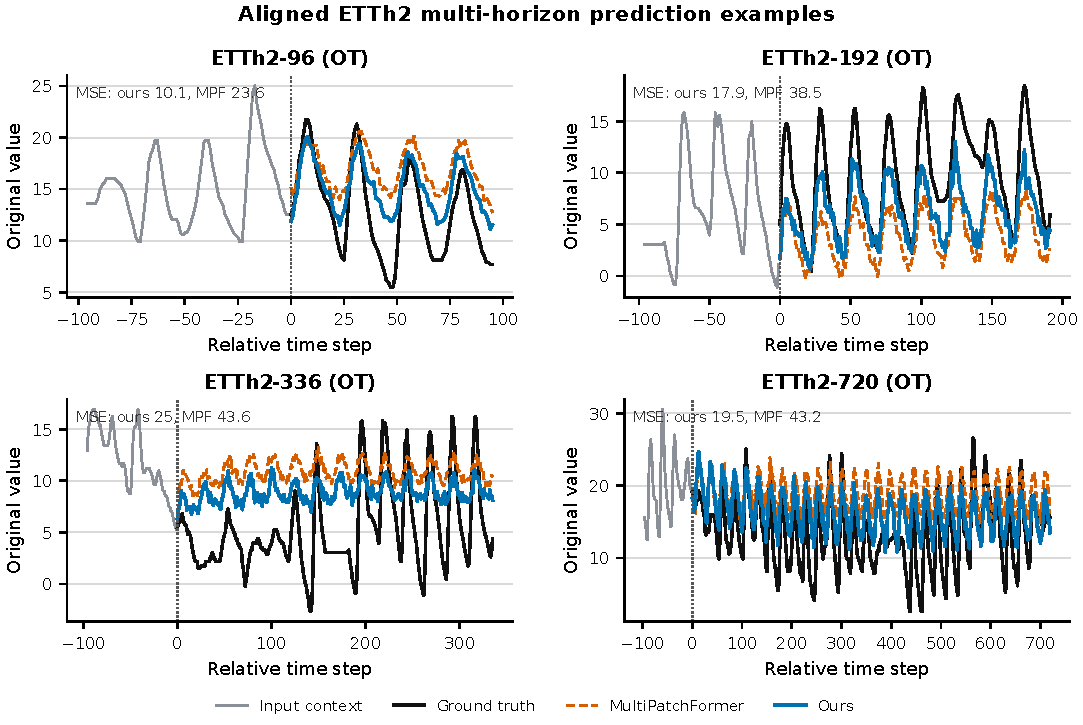
\includegraphics[width=0.95\textwidth]{figs/fig_etth2_multihorizon_prediction_comparison.pdf}
\caption{Aligned ETTh2 multi-horizon prediction examples. Each panel compares the input context, ground truth, FRWKV+ selected prediction, and MultiPatchFormer prediction on the same target channel and aligned test window. Window-level MSE values in the panels are computed on the original data scale for the displayed target channel only; they are qualitative window diagnostics and are not directly comparable across panels.}
\label{fig:prediction_examples}
\end{figure}

\subsection{Efficiency}
Table~\ref{tab:eff} compares the computational footprint of FRWKV, CrossBranchGate, and FRWKV+ on representative settings. FRWKV+ preserves the lightweight parameter scale of the FRWKV backbone: the parameter increase is about 0.01M relative to FRWKV in the reported settings, and peak training memory remains nearly unchanged. The additional periodic-position routing and trust branch mainly affects runtime, leading to a modest increase in training time per step in these measurements. Inference time remains comparable at this scale, although small differences should be interpreted with caution because they can be affected by hardware scheduling and implementation details.

These results support the intended design trade-off: FRWKV+ adds the Adaptive PhaseGate correction module without changing the overall memory profile of the frequency-space linear backbone. Its empirical benefit should therefore be interpreted together with the regime analysis in the matched ablation, where the added computation is most justified on datasets and horizons that benefit from adaptive periodic-position correction.

\begin{table}[t]
\centering
\caption{Efficiency comparison on representative settings.}
\label{tab:eff}
\scriptsize
\begin{tabular}{llcccc}
\toprule
Model & Dataset & Params(M) & Infer ms/step & Train ms/step & Peak train MB \\
\midrule
FRWKV & ETTh1-96 & 14.357 & 15.567 & 60.826 & 486.1 \\
CrossBranchGate & ETTh1-96 & 14.359 & 16.466 & 58.528 & 486.1 \\
FRWKV+ & ETTh1-96 & 14.369 & 14.132 & 68.590 & 487.5 \\
FRWKV & ETTh2-192 & 14.381 & 14.213 & 61.841 & 486.7 \\
CrossBranchGate & ETTh2-192 & 14.384 & 16.942 & 62.853 & 486.8 \\
FRWKV+ & ETTh2-192 & 14.393 & 14.998 & 69.489 & 488.0 \\
\bottomrule
\end{tabular}
\par\smallskip
\begin{minipage}{\textwidth}
\footnotesize \emph{Note:} Runtime values are local wall-clock measurements per step. They are intended to compare implementation-level overhead under the same environment rather than provide hardware-independent throughput claims.
\end{minipage}
\end{table}

Beyond the representative per-step comparison, we further profile the selected FRWKV+ recipes across all seven datasets and four prediction lengths. Table~\ref{tab:runtime_profile} reports a compact dataset-level summary of this completed single-seed profiling run. The placement follows the reporting pattern used by recent forecasting studies, where hardware-dependent runtime and memory diagnostics are discussed in the efficiency or complexity analysis, while detailed per-setting records are kept as supplementary evidence. These profiling results are used only to document computational behavior and training diagnostics; the statistical performance claims remain based on the benchmark tables and matched-seed ablation.

\begin{table}[t]
\centering
\caption{Single-seed runtime and loss profile of FRWKV+ across datasets.}
\label{tab:runtime_profile}
\scriptsize
\setlength{\tabcolsep}{3pt}
\begin{tabular}{lcccccc}
\toprule
Dataset & Epochs & Train(s) & Test(s) & Peak(MB) & Test loss & MSE/MAE \\
\midrule
ETTh1 & 20.0 & 302.4 & 1.14 & 595.5 & 0.0498 & 0.4386/0.4327 \\
ETTh2 & 22.5 & 325.0 & 1.15 & 602.5 & 0.0423 & 0.3664/0.3888 \\
ETTm1 & 15.0 & 887.3 & 4.96 & 1223.8 & 0.0430 & 0.3840/0.3866 \\
ETTm2 & 15.0 & 885.5 & 4.92 & 1221.3 & 0.0332 & 0.2768/0.3174 \\
Weather & 15.0 & 2600.9 & 11.86 & 2982.6 & 0.0261 & 0.2436/0.2643 \\
Exchange & 30.0 & 276.3 & 0.54 & 639.8 & 0.0347 & 0.3916/0.4190 \\
ILI & 46.0 & 96.6 & 0.13 & 405.1 & 0.1933 & 1.6338/0.7735 \\
\bottomrule
\end{tabular}
\par\smallskip
\begin{minipage}{\textwidth}
\footnotesize \emph{Note:} The profile uses seed 2024. Epochs, train time, test time, test loss, MSE, and MAE are averaged over the four horizons of each dataset. Peak(MB) reports the maximum peak allocated CUDA memory across the four horizons. Test loss is the same weighted sequence loss used for optimization, while MSE/MAE are the forecasting metrics. Detailed per-horizon measurements are retained as supplementary reproducibility records.
\end{minipage}
\end{table}

\subsection{Ablation on periodic-position variants}
Table~\ref{tab:ablation} reports the strict matched-seed FRWKV-family ablation. The study covers five variants, 28 dataset-horizon settings, and 16 shared seeds per setting, with complete records for all planned runs. This design removes seed mismatch from the internal comparison and allows us to summarize both setting-level winner coverage and dataset-level behavior.

\textbf{Observation 1: adaptive correction improves MSE coverage.}
Across the 28 settings, FRWKV+ obtains the largest MSE winner coverage, with eight MSE wins and seven MAE wins. This supports the intended role of periodic-position context as a useful correction signal for selected forecasting regimes.

\textbf{Observation 2: periodic correction should remain conservative.}
FRWKV obtains seven MSE wins and the largest MAE winner coverage, with twelve MAE wins. Average-rank results further show that FRWKV+ is not the best overall default under the matched protocol: its average ranks are 2.964 for MSE and 3.214 for MAE, while FRWKV obtains lower average ranks of 2.750 and 2.464. Thus, the matched ablation supports a selective-correction interpretation rather than a uniform-dominance claim.

\textbf{Observation 3: different datasets favor different correction regimes.}
The dataset-level averages reveal clear regime-dependent behavior. FRWKV+ is the best dataset-level variant on ETTh2 for both MSE and MAE, suggesting that adaptive periodic-position correction is most reliable in this regime. CrossBranchGate leads on ETTh1 and ILI, CrossBranchPhaseGate leads on ETTm1 and on ETTm2 MSE, FRWKV leads on Weather and on ETTm2 MAE, and FullContextDelta leads on Exchange. Together with Table~\ref{tab:ablation}, these outcomes indicate that periodic-position information is useful when admitted through adaptive trust, while simpler branch interaction, the original FRWKV gate, or fuller correction context can be preferable when the periodic cue is weaker, noisier, or more horizon-sensitive. Detailed matched-seed statistics, setting-level mean$\pm$std results, and paired comparison summaries are provided in the supplementary material.

\begin{table}[t]
\centering
\caption{Strict matched 16-seed dataset-level ablation within the FRWKV family.}
\label{tab:ablation}
\scriptsize
\setlength{\tabcolsep}{3pt}
\begin{tabular}{lccccc}
\toprule
Dataset & FRWKV+ & FullCtxDelta & PhaseGate & BranchGate & FRWKV \\
\midrule
ETTh1 & $0.4391/0.4323$ & $0.4384/0.4318$ & $0.4388/0.4321$ & $\mathbf{0.4376}/\mathbf{0.4317}$ & $0.4379/0.4318$ \\
ETTh2 & $\mathbf{0.3679}/\mathbf{0.3899}$ & $0.3691/0.3905$ & $0.3695/0.3906$ & $0.3685/0.3906$ & $0.3685/0.3901$ \\
ETTm1 & $0.3816/0.3854$ & $0.3812/0.3848$ & $\mathbf{0.3810}/\mathbf{0.3847}$ & $0.3819/0.3852$ & $0.3816/0.3848$ \\
ETTm2 & $0.2751/0.3164$ & $0.2754/0.3167$ & $\mathbf{0.2747}/0.3162$ & $0.2755/0.3166$ & $0.2751/\mathbf{0.3162}$ \\
Weather & $0.2439/0.2647$ & $0.2442/0.2648$ & $0.2440/0.2648$ & $0.2441/0.2648$ & $\mathbf{0.2439}/\mathbf{0.2646}$ \\
Exchange & $0.3950/0.4185$ & $\mathbf{0.3922}/\mathbf{0.4168}$ & $0.3998/0.4194$ & $0.4204/0.4254$ & $0.4011/0.4195$ \\
ILI & $1.6466/0.7758$ & $1.6410/0.7752$ & $1.6438/0.7758$ & $\mathbf{1.6373}/\mathbf{0.7736}$ & $1.6432/0.7758$ \\
\bottomrule
\end{tabular}
\par\smallskip
\begin{minipage}{\textwidth}
\footnotesize \emph{Note:} Each cell reports average MSE/MAE after equally averaging the four horizons of each dataset. All five variants use the same 16 seeds on all 28 dataset-horizon settings, and all planned records are complete. Bold values mark the best dataset-level average for each metric. FRWKV+ denotes the Adaptive PhaseGate variant, PhaseGate denotes CrossBranchPhaseGate, and BranchGate denotes CrossBranchGate.
\end{minipage}
\end{table}

\subsection{Discussion}
The matched-seed family ablation gives a more precise interpretation of FRWKV+ than a strongest-single-run table alone. Across the 28 dataset-horizon settings, FRWKV+ achieves the largest MSE winner coverage within the FRWKV family, with eight MSE wins, while FRWKV achieves the largest MAE winner coverage, with twelve MAE wins. The average-rank comparison further shows that FRWKV+ is not the strongest default choice under every metric: its average ranks are 2.964 on MSE and 3.214 on MAE, whereas FRWKV obtains 2.750 and 2.464, respectively. These results support a selective-correction view rather than a uniform-dominance view. Adaptive PhaseGate is useful when periodic-position cues provide reliable evidence for adjusting the real-imaginary branch interaction, but the same correction path should remain conservative when those cues are weak, noisy, or metric-sensitive.

The dataset-level winners clarify this regime-dependent behavior. ETTh2 is the clearest case where adaptive periodic-position correction is beneficial at the dataset level, suggesting that its periodic-position structure aligns well with the trust-controlled signed gate correction. By contrast, ETTh1 and ILI are better served by CrossBranchGate in the dataset-level averages, ETTm1 and ETTm2 MSE favor CrossBranchPhaseGate, Weather favors the original FRWKV on both averaged metrics, and Exchange favors FullContextDelta. These outcomes define the boundary conditions under which different correction contexts are preferable. Simpler branch interaction can be sufficient when the periodic cue is unstable, a fuller correction context can help when local period-position summaries are too narrow, and the original FRWKV gate can remain competitive when additional modulation mostly affects MAE-sensitive behavior.

These results suggest a conservative use pattern for FRWKV+. The model admits periodic-position information through signed, trust-controlled corrections, and is therefore best understood as an enhanced FRWKV variant for regimes where periodic-position context can reliably guide frequency-branch gates. This pattern is clearest in ETTh2 and in selected horizon-level wins. When the periodic-position signal is less reliable, the adaptive trust path is expected to suppress the correction and keep the representation close to simpler frequency-branch interactions. Future extensions should therefore focus on estimating periodic-position reliability more explicitly, reducing per-setting search, and learning when to select among branch-only, position-corrected, and fuller-context correction regimes.

\paragraph{Limitations.}
This study is intentionally scoped to seven standard long-term forecasting benchmarks: ETTh1, ETTh2, ETTm1, ETTm2, Weather, Exchange, and ILI. These datasets cover several commonly used forecasting regimes, but they do not exhaust the behavior of large-scale, high-dimensional, or strongly heterogeneous industrial time series. In particular, Traffic-like datasets and larger high-dimensional benchmarks remain important future test cases because they can stress cross-variable interaction, memory use, and the reliability of compact periodic-position summaries more severely than the datasets studied here.

A second limitation is that FRWKV+ is not the average-rank best variant in the matched-seed internal ablation. The matched 16-seed results show that FRWKV+ obtains the largest MSE winner coverage, but FRWKV has stronger average ranks and the largest MAE winner coverage. This means the evidence supports FRWKV+ as a selective periodic-position correction model with clear gains in selected regimes, rather than as a dominant default architecture across all metrics. The main comparison tables also use a selected-result reporting protocol for external benchmarking, whereas the mechanism-level conclusions rely on the matched-seed ablation. These two protocols answer different questions: the selected-result table summarizes the selected manuscript-level forecasting system under the external benchmark protocol, while the matched-seed ablation provides the fairer evidence for claims about FRWKV+, branch interaction, periodic-position correction, and adaptive trust.

Finally, the current adaptive trust mechanism learns when to admit periodic-position correction, but the reliability of the periodic-position signal is still estimated implicitly through the model rather than through an explicit reliability estimator. The dataset-level boundary cases suggest that such reliability varies across horizons, metrics, and datasets: ETTh2 is the clearest case where adaptive periodic-position correction is beneficial, while Weather, Exchange, ILI, and some ETT settings favor simpler branch interaction, the original FRWKV gate, or fuller correction context. Future work should make periodic-position reliability more explicit, reduce per-setting recipe search, and extend the evaluation to Traffic and other large high-dimensional datasets where the trade-off between compact periodic correction and fuller cross-variable context may become more pronounced.

\section{Conclusion}
We presented FRWKV+, a lightweight enhanced FRWKV model for frequency-space linear time series forecasting. Its Adaptive PhaseGate mechanism augments cross-branch real-imaginary frequency interaction with signed gate corrections derived from periodic-position context, and controls these corrections through adaptive trust scores. The matched 16-seed FRWKV-family analysis shows that FRWKV+ provides the largest MSE winner coverage across the 28 dataset-horizon settings and achieves its clearest dataset-level gains on ETTh2. At the same time, the results show regime-dependent behavior: CrossBranchGate, CrossBranchPhaseGate, FullContextDelta, and FRWKV each remain preferable on different datasets or metrics. These findings support the view that periodic-position information is valuable when used as a selective, trust-controlled correction signal, while its reliability varies across forecasting regimes. Future work should develop more principled estimators of periodic-position reliability, reduce per-setting tuning, and extend the analysis to larger and more heterogeneous forecasting datasets.

\section*{CRediT authorship contribution statement}
Dongyue Chen: Supervision, Project administration, Writing - review \& editing. Qingyuan Yang: Validation, Writing - review \& editing. Da Teng: Validation, Writing - review \& editing. Junhua Xiao: Validation, Writing - review \& editing. Jiaji Pan: Validation, Writing - review \& editing. Shizhuo Deng: Conceptualization, Methodology, Software, Formal analysis, Writing - original draft.

\section*{Funding}
This work was supported by the National Key R\&D Program of China (2024YFB4710900) and the Guangdong Basic and Applied Basic Research Foundation under Grant 2024A1515010244.

\section*{Declaration of competing interest}
The authors declare that they have no known competing financial interests or personal relationships that could have appeared to influence the work reported in this paper.

\section*{Data availability}
The benchmark datasets used in this study are publicly available long-term forecasting datasets. The code, configuration files, and result aggregation scripts supporting this study will be made available in a public repository upon acceptance.

\section*{Declaration of generative AI use}
During the preparation of this work, the authors used generative artificial intelligence tools to assist with coding tasks related to experiment organization and result-file processing. The authors reviewed and verified the AI-assisted coding outputs and take full responsibility for the content of the published article.

\begin{thebibliography}{00}
\bibitem{kim2022revin} Kim T, Kim J, Tae Y, Park C, Choi J, Choo J. Reversible instance normalization for accurate time-series forecasting against distribution shift. In: ICLR; 2022.
\bibitem{zhou2021informer} Zhou H, Zhang S, Peng J, Huang Y, Li J, Xiong H, Zhang W. Informer: beyond efficient Transformer for long sequence time-series forecasting. Proceedings of the AAAI Conference on Artificial Intelligence. 2021;35(12):11106--11115.
\bibitem{wu2021autoformer} Wu H, Xu J, Wang J, Long M. Autoformer: decomposition Transformers with auto-correlation for long-term series forecasting. In: Advances in Neural Information Processing Systems; 2021.
\bibitem{zhou2022fedformer} Zhou T, Ma Z, Wen Q, Wang X, Sun L, Jin R. FEDformer: frequency enhanced decomposed Transformer for long-term series forecasting. In: Proceedings of the 39th International Conference on Machine Learning; 2022. p. 27268--27286.
\bibitem{nie2023patchtst} Nie Y, Nguyen NH, Sinthong P, Kalagnanam J. A time series is worth 64 words: long-term forecasting with transformers. In: ICLR; 2023.
\bibitem{wu2023timesnet} Wu H, Hu T, Liu Y, Zhou H, Wang J, Long M. TimesNet: temporal 2D-variation modeling for general time series analysis. In: ICLR; 2023.
\bibitem{wang2024timemixer} Wang S, Wu H, Shi H, Zhu H, Long M. TimeMixer: decomposable multiscale mixing for time series forecasting. In: ICLR; 2024.
\bibitem{liu2024itransformer} Liu Y, Hu T, Zhang H, Wu H, Wang S, Ma L, Long M. iTransformer: inverted transformers are effective for time series forecasting. In: ICLR; 2024.
\bibitem{zeng2023dlinear} Zeng A, Chen M, Zhang L, Xu Q. Are transformers effective for time series forecasting? In: AAAI; 2023.
\bibitem{peng2023rwkv} Peng B, Alcaide E, Anthony Q, Albalak A, Arcadinho S, Biderman S, et al. RWKV: reinventing RNNs for the Transformer era. In: Findings of the Association for Computational Linguistics: EMNLP 2023; 2023. p. 14048--14077.
\bibitem{gu2023mamba} Gu A, Dao T. Mamba: linear-time sequence modeling with selective state spaces. arXiv preprint arXiv:2312.00752; 2023.
\bibitem{yang2025frwkv} Yang Q, Deng S, Chen D, Teng D, Gan Z. FRWKV: frequency-domain linear attention for long-term time series forecasting. arXiv preprint arXiv:2512.07539; 2025. doi:10.48550/arXiv.2512.07539.
\bibitem{hou2024rwkvts} Hou H, Yu FR. RWKV-TS: beyond traditional recurrent neural network for time series tasks. arXiv preprint arXiv:2401.09093; 2024.
\bibitem{wang2025smamba} Wang Z, Kong F, Feng S, Wang M, Yang X, Zhao H, Wang D, Zhang Y. Is Mamba effective for time series forecasting? Neurocomputing. 2025;619:129178.
\bibitem{chowdhury2025t3time} Chowdhury AM, Akter R, Arib SH. T3Time: tri-modal time series forecasting via adaptive multi-head alignment and residual fusion. arXiv preprint arXiv:2508.04251; 2025.
\bibitem{liu2025timecma} Liu C, Xu Q, Miao H, Yang S, Zhang L, Long C, Li Z, Zhao R. TimeCMA: towards LLM-empowered multivariate time series forecasting via cross-modality alignment. In: Proceedings of the AAAI Conference on Artificial Intelligence; 2025. p. 18780--18788.
\bibitem{jin2024timellm} Jin M, Wang S, Ma L, Chu Z, Zhang JY, Shi X, Chen P-Y, Liang Y, Li Y-F, Pan S, Wen Q. Time-LLM: time series forecasting by reprogramming large language models. In: ICLR; 2024.
\bibitem{ansari2025chronos2} Ansari AF, Shchur O, Kuken J, Auer A, Han B, Mercado P, Rangapuram SS, Shen H, Stella L, Zhang X, Goswami M, Kapoor S, Maddix DC, Guerron P, Hu T, Yin J, Erickson N, Desai PM, Wang H, Rangwala H, Karypis G, Wang Y, Bohlke-Schneider M. Chronos-2: from univariate to universal forecasting. arXiv preprint arXiv:2510.15821; 2025.
\bibitem{liu2024unitime} Liu X, Hu J, Li Y, Diao S, Liang Y, Hooi B, Zimmermann R. UniTime: a language-empowered unified model for cross-domain time series forecasting. In: Proceedings of the ACM Web Conference; 2024.
\bibitem{yi2023frets} Yi K, Zhang Q, Fan W, Wang S, Wang P, He H, Lian D, An N, Cao L, Niu Z. Frequency-domain MLPs are more effective learners in time series forecasting. In: Advances in Neural Information Processing Systems; 2023.
\bibitem{naghashi2025multipatchformer} Naghashi V, Boukadoum M, Diallo AB. A multiscale model for multivariate time series forecasting. Scientific Reports. 2025;15:1565.
\bibitem{niu2026phaseformer} Niu Y, Deng J, Tong Y. PhaseFormer: from patches to phases for efficient and effective time series forecasting. In: ICLR; 2026.
\end{thebibliography}

\end{document}
